\documentclass[journal,twoside,web]{ieeecolor}

\usepackage{tmi}
\def\BibTeX{{\rm B\kern-.05em{\sc i\kern-.025em b}\kern-.08em
    T\kern-.1667em\lower.7ex\hbox{E}\kern-.125emX}}
\markboth{\journalname, VOL. XX, NO. XX, XXXX 2020}
{Schramm \MakeLowercase{\textit{et al.}}: Foo bar}


\usepackage{amsmath,amssymb,amsfonts}
\usepackage{graphicx}
\usepackage{textcomp}

\usepackage{algpseudocode}
\usepackage{grffile}
\usepackage[font={footnotesize}]{caption}
\usepackage{subcaption}

\usepackage[backend=bibtex,minnames=3,maxnames=3,isbn=false,url=false,eprint=false,giveninits=true,sorting=none,citestyle=numeric-comp]{biblatex}
\addbibresource{gs.bib}

% define float env for algorithm
\usepackage{float}
\floatstyle{ruled}
\newfloat{algorithm}{h}{loa}
\floatname{algorithm}{Algorithm}

% custom definitions
\DeclareMathOperator{\proj}{proj}
\DeclareMathOperator{\prox}{prox}
\DeclareMathOperator*{\argmin}{argmin}


\AtBeginBibliography{\small}

\pdfoutput=1


%-------------------------------------------------------------------------------------------------------

\begin{document}

\title{Fast and memory-efficient reconstruction of sparse time-of-flight PET data in listmode with non-smooth priors
}

\author{Georg Schramm and Martin Holler}

\thanks{This paragraph of the first footnote will contain the date on which
you submitted your paper for review. It will also contain support information,
including sponsor and financial support acknowledgment. For example, 
``This work was supported in part by the U.S. Department of Commerce under Grant BS123456.'' }
\thanks{The next few paragraphs should contain the authors' current affiliations,
including current address and e-mail. For example, F. A. Author is with the
National Institute of Standards and Technology, Boulder, CO 80305 USA (e-mail:author@boulder.nist.gov). }


\maketitle

\begin{abstract}
%auto-ignore
Complete time of flight (TOF) sinograms of state-of-the-art TOF PET scanners have a large memory 
footprint.
Currently, they contain ${\sim}4{\cdot}10^9$ data bins which amount to ${\sim}17$\,GB 
in 32\,bit floating point precision.
Moreover, their size will continue to increase with advances in the 
achievable detector TOF resolution and increases in the axial field of view.
Using iterative algorithms to reconstruct such enormous TOF sinograms becomes increasingly
challenging due to the memory requirements and the computation time needed to evaluate the
forward model for every data bin.
This is especially true for more advanced optimization algorithms such as the
stochastic primal-dual hybrid gradient (SPDHG) algorithm which allows for the use of non-smooth priors
for regularization using subsets with guaranteed convergence.
SPDHG requires the storage of additional sinograms in memory, which severely limits
its application to data sets from state-of-the-art TOF PET systems using conventional
computing hardware.

Motivated by the generally sparse nature of the TOF sinograms, we propose and analyze a new 
listmode (LM) extension of the SPDHG algorithm  for image reconstruction of sparse data 
following a Poisson distribution.
Based on realistic 2D and 3D simulations \added{as well as a real dataset acquired on a 
state-of-the-art TOF PET/CT system}, we show that the speed of convergence of the proposed 
LM-SPDHG is equivalent the original SPDHG operating on binned data (TOF sinograms).
However, we find that for a TOF PET system with 400\,ps TOF resolution and 25\,cm axial FOV,
the proposed LM-SPDHG reduces the required memory from approximately 56\,GB to
0.7\,GB for a short dynamic frame with $10^7$ prompt coincidences and to 12.4\,GB for a long 
static acquisition with $5\cdot10^8$ prompt coincidences.

In contrast to SPDHG, the reduced memory requirements of LM-SPDHG enables 
a pure GPU implementation on state-of-the-art GPUs - avoiding memory transfers
between host and GPU - which will substantially accelerate reconstruction times.
This in turn will allow the application of LM-SPDHG in routine clinical practice where short
reconstruction times are crucial.

\end{abstract}

\begin{IEEEkeywords}
Enter about five key words or phrases in alphabetical order, separated by commas.
\end{IEEEkeywords}

%\section*{Summary}
%
%\begin{itemize}
%\item SPDHG excellent alg for non-smooth priors, but only sinogram
%\item modern TOF PET data is extremly sparse (Figure) -> SPDHG inefficient
%      in terms of memory and speed
%\item LM projections are much faster than sino projections for usual count levels
%      (Table)
%\item propose LM-SPDHG that solves both issues
%\item 1st step: better init
%\item 2nd step: rewrite SPDHG in terms of LM updates
%\end{itemize}

%%%%%%%%%%%%%%%%%%%%%%%%%%%%%%%%%%%%%%%%%%%%%%%%%%%%%%%%%%%%%%%%%%%%%%%%%%%%%%%%%%%%%%%%%%%%%%%%%%%%%%%%
%%%%%%%%%%%%%%%%%%%%%%%%%%%%%%%%%%%%%%%%%%%%%%%%%%%%%%%%%%%%%%%%%%%%%%%%%%%%%%%%%%%%%%%%%%%%%%%%%%%%%%%%
%%%%%%%%%%%%%%%%%%%%%%%%%%%%%%%%%%%%%%%%%%%%%%%%%%%%%%%%%%%%%%%%%%%%%%%%%%%%%%%%%%%%%%%%%%%%%%%%%%%%%%%%
%%%%%%%%%%%%%%%%%%%%%%%%%%%%%%%%%%%%%%%%%%%%%%%%%%%%%%%%%%%%%%%%%%%%%%%%%%%%%%%%%%%%%%%%%%%%%%%%%%%%%%%%
\newcommand{\todo}[1]{\textcolor{red}{ #1}}
\section{Introduction}

% add importance of fast recons

A major challenge of image reconstruction in positron emission tomography (PET)
is noise suppression since the acquired emission data suffer from high levels of Poisson
noise due to limitations in acquisition time, injectable dose and scanner sensitivity.
To limit the transfer of the data noise into the image during model-based iterative
reconstruction (MBIR), different strategies exist. 
One possibility is to add a ``smoothing'' prior to the data fidelity term in the cost
function that is being optimized.
In general, we can formulate the resulting optimization problem for PET image reconstruction as
%
\begin{equation}
\argmin _{x\geq 0} \sum_{i=1}^{m} \underbrace{(Px + s)_i -  d_i \log \left( (Px + s)_i \right)}_{D_i((Px+s)_i)} + \, \beta R(Kx),
\label{eq:primal}
\end{equation}
%
where $x$ is the PET image to be reconstructed, $P$ is the time of flight (TOF) 
forward model including the effects
of attenuation, normalization and limited spatial resolution, $d$ are the 
acquired prompt TOF coincidences (the emission sinogram), 
and $s$ are additive contaminations including random and scattered coincidences. 
$\sum_{i=1}^m D_i(x)$ is the negative Poisson log-likelihood, $i$ is the index of the data (TOF sinogram)
bin and $m$ is the total number of data bins.
$R(K\cdot)$ is the ``smoothing prior'' consisting of a generic linear operator $K$ that calculates 
local differences and a proper, convex, lower-semicontinous function $R$.
The level of regularization is controlled by the non-negative scalar factor $\beta$.
A specific example for $K$ would be the gradient operator $\nabla$, e.g. approximated by finite forward 
differences in the discretized setting.
Combining the gradient operator for $K$ with the mixed L2-L1 norm for $R$ leads to the well-known 
Total Variation (TV) prior \cite{Rudin1992}.

The TV prior, as well as many other advanced smoothing priors aiming for edge-preservation 
such as e.g. Total Generalized Variation (TGV) 
\cite{Bredies2010}, Joint T(G)V \cite{Rigie2015,Knoll2016}
Parallel Level Sets \cite{Ehrhardt2016a,Schramm2017} or directional Total Variation (DTV)
\cite{Ehrhardt2016}, require the use of non-smooth functions for $R$ as instrumental building block.
This prevents the use of simple and efficient 
purely gradient-based optimization algorithms to solve \eqref{eq:primal}.


%Unfortunately, many advanced smoothing priors aiming for edge-preservation 
%such as e.g. TV \cite{Rudin1992}, Total Generalized Variation (TGV) 
%\cite{Bredies2010}, Joint T(G)V \cite{Rigie2015,Knoll2016}
%Parallel Level Sets \cite{Ehrhardt2016a,Schramm2017} or directional Total Variation (DTV)
%\cite{Ehrhardt2016} use non-smooth functions for $R$ which permits the use of simple and efficient 
%purely gradient-based optimization algorithms to solve \eqref{eq:primal}.

\subsection*{PDHG and SPDHG for PET reconstruction with non-smooth priors}

Using the fact that $D(x) = \sum_i D_i(x)$ and $\beta R(x)$ are convex functions and thus are
equal to their convex biconjugates 
$D^{**}(Px + s) = \sup_y \langle Px + s, y \rangle - \sum_{i=1}^{m} D_i^*(y_i)$ 
and $(\beta R)^{**}(Kx) = \sup_w \langle Kx, w \rangle - (\beta R)^*(w)$, respectively, 
where $D_i^*$ and $(\beta R)^*$ are the convex conjugates,
and that $(\beta R)^*(w) = \beta R^*(w / \beta)$, 
we can rewrite \eqref{eq:primal} as the saddle point problem
%
\begin{equation}
\argmin_{x\geq 0} \, \sup_{y,w} \,  \langle Px + s, y \rangle + \langle Kx, w \rangle - \sum_{i=1}^{m} D_i^*(y_i) - \beta R^*(w/\beta) ,
\label{eq:saddle}
\end{equation}
%
introducing the dual variables $y$ and $w$, and the convex dual of the Poisson log-likelihood given as
%
\begin{equation}
D_i^*(y_i) =
\begin{cases}
-d_i + d_i \log \left( \frac{d_i}{1-y_i} \right) & \text{if } y_i < 1 \\
\infty & \text{else} \ .
\end{cases}
\end{equation}
for $d_i >0$ and $D_i^*(y_i) = 0$ if $y_i \leq 1$ and $D_i^*(y_i) = \infty$ if $y_i >1$ in the other case.
%
Under mild assumptions on $R$, which hold for all of above-mentioned smoothing priors, Problem \eqref{eq:saddle} is equivalent to \eqref{eq:primal} and
%Problem \eqref{eq:saddle}, 
can be solved even for non-smooth priors using the generic primal-dual hybrid gradient (PDHG) 
algorithm by Chambolle and Pock \cite{Chambolle2011}.
PDHG is in iterative algorithm that requires the evaluation of the complete forward and adjoint operator
in every update.
The usage of the original PDHG algorithm to solve \eqref{eq:saddle} for real-world state-of-the-art
TOF PET systems, however, usually results in extremely long computation times, 
because the evaluation of $P$ and $P^T$
for state-of-the-art TOF PET systems is computationally very demanding, and 
because several hundreds to thousands of updates are needed to obtain reasonable convergence.

To overcome this limitation, Chambolle et al. published a stochastic extension of PDHG called SPDHG 
for saddle point problems that are separable in the dual variable in 2018 \cite{Chambolle2018}.
In contrast to PDHG, SPDHG has the advantage that the complete forward and adjoint operator are
split into $n$ subsets, and that, in every update, only a random subset of the forward
and adjoint operator chosen according to a probability $p_k$ have to be evaluated.
In \cite{Ehrhardt2019}, Ehrhardt et al. applied SPDHG to 3D non-TOF PET reconstruction with TV-like
priors and showed that around 10 complete projections and back projections are sufficient 
to obtain reasonable convergence using SPDHG with 252 subsets.
Moreover, the authors also demonstrated that preconditioning further accelerates convergence.
The resulting SPDHG algorithm to solve \eqref{eq:saddle} is summarized in Algorithm \ref{alg:spdhg},
where the proximal operator of the convex conjugate of the negative Poisson log-likehood $D_i^*$ 
can be calculated point-wise and is given by
%
\begin{equation}
\begin{split}
(\prox_{D_i^*}^{S}(y))_i &= \prox_{D_i^*}^{S}(y_i) \\ 
&= \frac{1}{2} \left(y_i + 1 - \sqrt{ (y_i-1)^2 + 4 S_i d_i} \right) \ .
\end{split}
\label{eq:proxD}
\end{equation} 
%
The proximal operator for $R^*$, obviously depends on the choice of $R$ but can be also efficiently 
computed using point-wise operations for many popular choices of $R$.
As mentioned in \cite{Ehrhardt2019}, Algorithm \ref{alg:spdhg} converges if we use the preconditioned
step sizes
%
\[ S_k = \gamma \, \text{diag}(\frac{\rho}{P_k 1} )\qquad  T_k = \gamma^{-1} \text{diag}(\frac{\rho p_k}{P^T_k 1}) \ , \]
% 
and
%
\[ S_{n+1} = \gamma \, \frac{\rho}{\|K\|} \qquad T_{n+1} = \gamma^{-1} \frac{p_i\rho}{\|K\|} \ , \]
%
setting $T = \min_{k=1,\ldots,n+1} T_k$ pointwise, and choosing $\rho<1$ and $\gamma>0$.
%
\begin{algorithm}[t]
\begin{algorithmic}[1]
\small
\State \textbf{Initialize} $x(=0),y(=0),(w=0)$, $(S_i)_i,T,(p_i)_i$,
\State $\overline{z} = z = P^T y + K^T w$
\Repeat
	\State $x \gets \proj_{\geq 0} (x - T \overline{z})$
	\State Select $i \in \{ 1,\ldots,n+1\} $ randomly according to $(p_i)_i$
  \If{$i \leq n$}
	\State $y_i^+ \gets \prox_{D_i^*}^{S_i} ( y_i + S_i  ( P_i x + s_i))$
	\State $\delta z \gets P_i^T (y_i^+ - y_i)$
	\State $y_i \gets y_i^+$
  \Else
	\State $w^+ \gets \beta \prox_{R^*}^{S_i/\beta} ((w + S_i  K x)/\beta)$
	\State $\delta z \gets K^T (w^+ - w)$
	\State $w \gets w^+$
  \EndIf
	\State $z \gets z + \delta z$
	\State $\overline{z} \gets  z + (\delta z/p_i)$
\Until{stopping criterion fulfilled}
\State \Return{$x$}
%\EndFunction
\end{algorithmic}
\caption{SPDHG for PET reconstruction \cite{Ehrhardt2019}}
\label{alg:spdhg}
\end{algorithm}
%

\subsection*{Limitations of PDHG and SPDHG for PET reconstruction}

Whilst SPDHG is a big step forward for an efficient solution of \eqref{eq:saddle}
in terms of computational speed, SPDHG also comes with two main limitations.
Firsts, as discussed in Remark 2 of \cite{Ehrhardt2019}, 
a potential drawback of SPDHG is that it requires keeping at least one more complete 
(TOF) sinogram in memory (the dual variable $y$). 
Moreover, if the proposed preconditioning is used, a second complete (TOF) sinogram
(the sequence of step sizes $(S_k)_{k=1}^n$) needs to be stored in memory.
Storing one or two extra sinograms in memory of modern computers is not a major problem for static 
single-bed non-TOF PET data, where sinogram sizes are relatively small.
However, for simultaneous multi-bed, dynamic or TOF PET data, the size of the complete data sinograms
can be become problematic.
This issue gets even more severe when aiming for a complete GPU implementation 
of Algorithm \ref{alg:spdhg} since the available memory on state-of-the-art GPUs is nowadays
much smaller compared to CPUs.

As an example, for a TOF PET scanner with 25\,cm axial FOV and a TOF resolution of ca. 400\,ps, 
a complete unmashed static TOF sinogram for one bed position 
has approximately $4.4\cdot10^9$ data bins, requiring ca. 17\,GB of memory in 32\,bit floating
point precision.
Note that with improved TOF resolution and increasing axial field of view (e.g. total body 
PET scanners), the memory required to store a complete TOF sinogram will continue to 
substantially increase in the future.

Second, PDHG and SPDHG only work with ``binned'' data.
In the case of TOF PET reconstruction, that means that the acquired raw listmode data first needs to be
binned into TOF sinograms and that $P$ and $P^T$ need to be evaluated using
sinogram projectors.
For most acquisitions with modern TOF PET scanners, this is inefficient both in terms of memory and
computational time since the TOF emission data is extremely sparse.
In contrast, storage and processing of the data in listmode format (event by event) is usually 
more efficient.

\subsection*{Sparsity of TOF PET data}

Compared to non-TOF PET emission sinograms, TOF PET emission sinograms of most acquisitions
with state-of-the-art TOF PET scanners are extremely sparse.
This is because every geometrical line of response (LOR) has to be subdivided into
several small TOF bins.
To achieve sufficient sampling of the TOF information, the number of TOF bins has to be
inversely proportional to the TOF resolution of the scanner. 
Consequently, for a fixed number of acquired prompt coincidences, the sparsity of the
sinogram is proportional to the TOF resolution.

As an example, for a typical 80\,s acquisition of a liver bed position in an FDG scan with 
an injected dose of around 323\,MBq acquired 60\,min p.i. on a state-of-the-art TOF PET/CT scanner with
20\,cm axial FOV, more than 94\% of the data (TOF sinogram) bins are empty.
An example that demonstrates this extreme sparsity of TOF sinograms is shown in Fig.~\ref{fig:sparsity}.
For shorter frames, as present, e.g., in the early phase of dynamic scans or when respiratory
or cardiac gating is used, the fraction of empty bins can even higher.

Note that we expect that the sparsity of the TOF emission data of future PET systems will increase 
faster than linear compared to the improvement of the TOF resolution.
This is because with better TOF resolution, every detected event carries more information such
that fewer detected events are needed to reconstruct images with the similar 
variance \cite{Tomitani1981}.

\begin{figure}
  \centering
    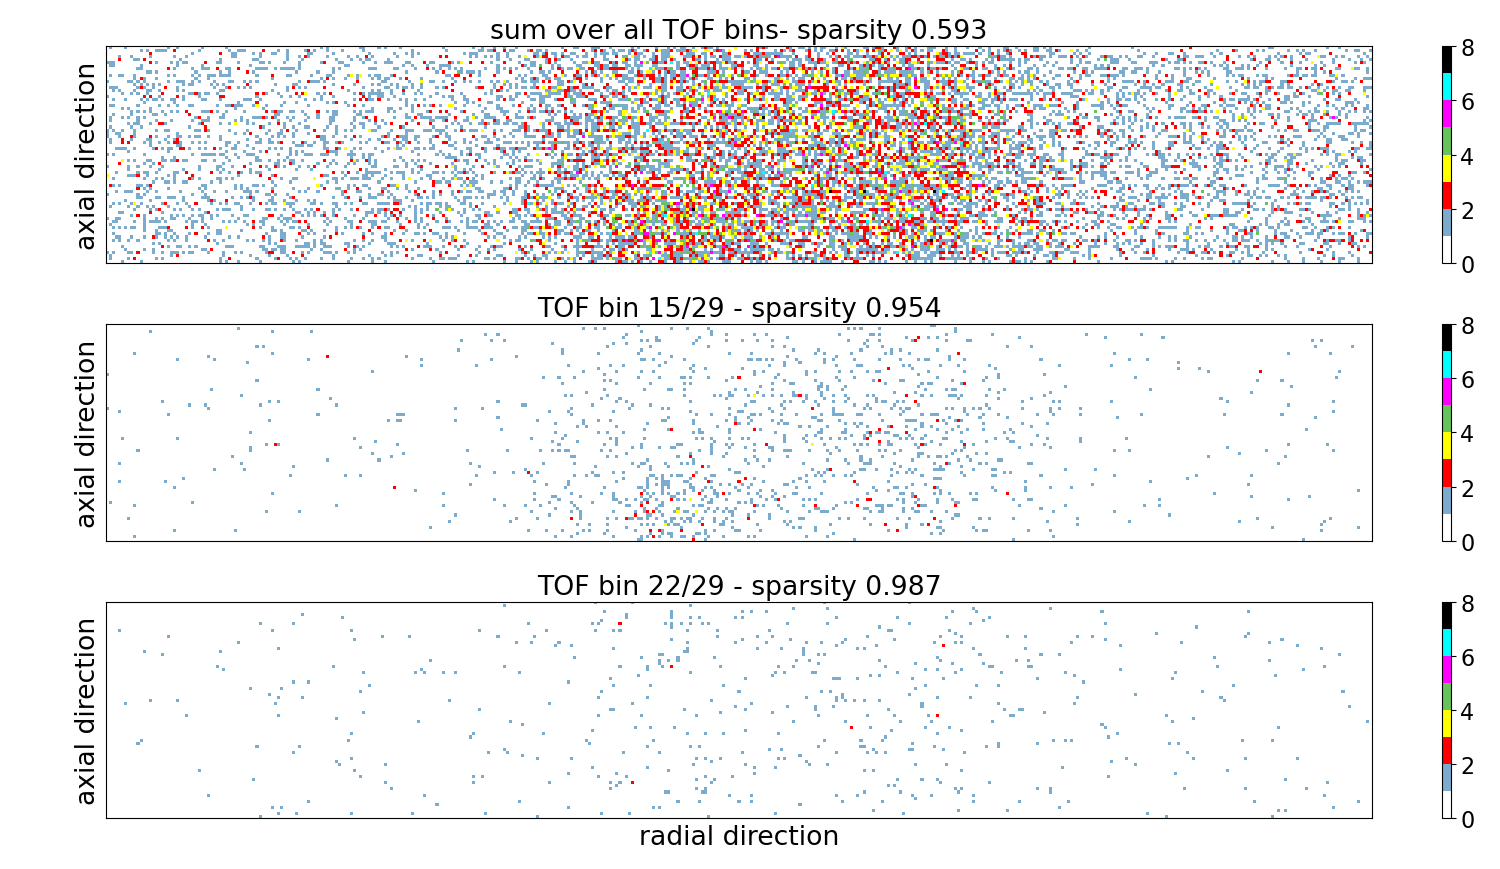
\includegraphics[width=1.0\columnwidth]{./figs/sparsity.png}
  \caption{Representative slices through a single view of an emission sinogram of a 
  80s [\textsuperscript{18}F]FDG acquisition of a liver bed position. 
  The scan was acquired 1\,h post injection with an injected dose of 323\,MBq on
  a GE DMI PET/CT with a TOF resolution of 400\,ps (29 TOF bins). 
  The horizontal and vertical axis represent the radial and axial direction (direct planes only), 
  respectively. 
  (top) sum over all TOF bins. (middle) central TOF bin 15/29 with 94\% empty bins. 
  (bottom) TOF bin 22/29 with 97\% empty bins.}

  \label{fig:sparsity}
\end{figure}


\subsection*{Contributions and Aim}

To improve the efficiency of SPDHG in terms of required memory and computation time when reconstructing 
sparse TOF PET data, we propose and analyze a listmode version of the SPDHG algorithm  called
LM-SPDHG that allows event-by-event processing using dedicated listmode forward and back projectors.
We first derive LM-SPDHG from SPDHG and show that the convergence of LM-SPDHG is as 
fast as the convergence of SPDHG based on dedicated numeric examples in 2D.
Moreover, we analyze the memory requirements for LM-SPDHG compared to SPDHG for typical scans 
acquired on state-of-the-art TOF scanners.

We emphasize that the focus of this work is not on finding the
optimal (non-smooth) prior or prior strength for a given clinical task in PET imaging.
Instead, we aim to provide a framework enabling fast and memory efficient reconstruction of 
sparse TOF PET listmode data which will finally facilitate future research on the use of
(non-smooth) priors in PET reconstruction. 


\section{Theory and Algorithms}

Before deriving LM-SPDHG, the next subsection first of all shows how to reduce the memory 
requirements of SPDHG when reconstructing sparse TOF sinograms. 

\subsection*{Memory-efficient SPDHG for sparse TOF sinograms}

As shown in \cite{Schramm2021}, the memory requirements for SPDHG can be substantially reduced by 
choosing a better initialization of the dual variable $y$.

From Eq.~(\ref{eq:proxD}) we can observe that for data bins $i$ where $d_i = 0$ 
(bins in the TOF emission sinogram with zero counts), 
$\prox_{D_i^*}(a_i) = 1$ for $a_i \geq 1$ and $\prox_{D_i^*}(a_i) = a_i$ 
otherwise. 
Moreover, provided that $y_i \geq 1$, we see that $ a_i = y_i + S_i (P_i x + s_i) \geq 1$ 
since all other quantities are non-negative. 
Consequently, if we initialize all bins of $y$ where the data sinogram $d$ equals zero with one, 
these bins of $y$ remain $1$ during all iterations. 
This in turn means that these bins do not contribute to the update of $\delta z$, $z$, $\bar{z}$, 
and $x$, since only the difference between
$y$ and $y^+$ is backprojected in line 8 of Algorithm~\ref{alg:spdhg} meaning that all
bins without data do not have to be kept in memory during the iteration loop (lines 3 until 17). 
The only place where the empty data bins contribute is the initialization of $z$ and $\bar{z}$
in line 2.
However, this single back projection can be split into smaller chunks to also reduce
the required memory of this step.

While at a first glance, the initialization of $y$ proposed above might seem artificial, in fact it corresponds directly choosing the optimal value for those $y_i$ where $d_i=0$. To see this, note that an optimal solution $(\hat{x},\hat{y},\hat{w})$ of \eqref{eq:saddle}  in particular needs to satisfy the optimality condition
\begin{equation}
P \hat{x} \in  \partial D^*(\hat{y}),
\end{equation}
where $\partial D^*$ is the subdifferential of $D^*$. Since this is equivalent to $\hat{y} \in  \partial D(P \hat{x})$, and since $D$ (the negative Poisson log likelihood) is differentiable and $P\hat{x}$, this leads
to the condition
\begin{equation}
\hat{y} = 1 - \frac{d}{P\hat{x} + s} \ ,
\label{eq:yinit}
\end{equation}
where the division is to be understood point-wise. With this we see that the proposed initialization corresponds to right away choosing the optimal value for $y_i $ where $d_i=0$, which is known explicitly in this case.

%At a first glance, the initialization of $y$ proposed above seems very artificial.
%But, if we construct a better initialization $y^0$ in a way such that it is the solution of our
%saddle point problem \eqref{eq:saddle} for a fixed initial $x^0$, it has to satisfy
%%
%\begin{equation}
%\langle P x^0, y^0 \rangle - D^*(y^0) = D(Px^0 + s) \ ,
%\end{equation}
%%
%which is the case when
%%
%\begin{equation}
%y^0 \in \partial D(Px + s) |_{x^0} \ .
%\end{equation}
%%
%Since $D$ (the negative Poisson log likelihood) is differentiable, this leads
%to the condition
%\begin{equation}
%y^0 = 1 - \frac{d}{Px^0 + s} \ ,
%\label{eq:yinit}
%\end{equation}
%where the division is to be understood point-wise.
%We see that under this condition, $y^0$ is indeed one in bins where $d$ is zero,
%irrespective of the choice of $x^0$.
As argued above, this improved initialization of $y$ naturally reduces the 
memory requirements of SPDHG and also improves the speed of convergence when a
``warm start'' for $x^0$ is chosen. 
The latter can, e.g., be achieved by applying one iteration
and a reasonable amount of subsets of the EM-TV algorithm \cite{Sawatzky2008, Burger2008}.
Since in EM-TV every update is split into a classical EM step followed by a weighted denoising
optimization problem in image space, EM-TV can be used in listmode as well by simply
modifying the EM step.

\subsection*{Listmode SPDHG}

As indicated by the name, emission data in listmode format are a chronological list $N$ of detected 
events $e \in N$, where each event is characterized by a small set of (integer) numbers 
(e.g. the number of the two detectors, the discretized TOF difference, and a time stamp).
To process the listmode data during reconstruction without binning it into a sinogram,
we introduce the listmode forward operator $P^{LM}_N$ mapping the image data $x$ to a 
data-vector of dimension $|N|$ via \[ (P^{LM}_N x)_e  = (Px)_{i_e} , \text{ for each }e \in N,\]
where $i_e$ is the sinogram bin in which event $e$ was detected.

Re-writing the gradient of the negative Poisson log likelihood using listmode data and the
listmode operators is straight forward, such that any gradient-based PET reconstruction algorithm 
can be easily adapted to listmode data.

For a Bayesian approach with prior $R(K \cdot)$ as in \eqref{eq:primal} this is less immediate, 
but we can show that indeed \eqref{eq:primal} can be equivalently re-written to a minimization 
problem involving only the listmode forward operator that is of the same form as \eqref{eq:primal}. 
This allows us to extend the SPDHG algorithm for listmode data and yields the algorithm as shown 
in Algorithm~\ref{alg:lmspdhg}.


%However, for SPDHG - which has the advantage of being able to handle non-smooth priors and
%has guaranteed convergence, an adaptation to listmode data is more complicated.
%Our proposed listmode SPDHG algorithm (LM-SPDHG) solves those complications and is shown in 
%Algorithm~\ref{alg:lmspdhg}.

\begin{algorithm}[t]
\begin{algorithmic}[1]
\small
\State \textbf{Input} event list $N$, contamination list $s_N$
\State \textbf{Calculate} event counts $\mu_e$ for each e in $N$ (see text)
\State \textbf{Initialize} $x,w,(S_i)_i,T,(p_i)_i$
\State \textbf{Initialize} list $y_{N} = 1 - (\mu_N /(P^{LM}_{N} x + s_{N}))$ 
\State \textbf{Preprocessing} $\overline{z} = z = {P^T} 1 - {P^{LM}}^T (y_N-1)/\mu_N + K^T w$ %(see \eqref{eq:zinit_lm} and text)
\State \textbf{Split} lists $N$, $s_N$ and $y_N$ into $n$ sublists $N_i$, $y_{N_i}$ and $s_{N_i}$
\Repeat
	\State $x \gets \proj_{\geq 0} (x - T \overline{z})$
	\State Select $i \in \{1,\ldots,n+1\}$ randomly according to $(p_i)_i$
  \If{$i \leq n$}
	  \State $y_{N_i}^+ \gets \prox_{D^*}^{S_i} \left( y_{N_i} + S_i \left(P^{LM}_{N_i} x + s_{N_i} \right) \right)$
	  \State $\delta z \gets {P^{LM}_{N_i}}^T \left(\frac{y_{N_i}^+ - y_{N_i}}{\mu_{N_i}}\right)$
	  \State $y_{N_i} \gets y_{N_i}^+$
  \Else
	  \State $w^+ \gets \beta \prox_{R^*}^{S_i/\beta} ((w + S_i  K x)/\beta)$
	  \State $\delta z \gets K^T \left(w^+ - w\right)$
	  \State $w \gets w^+$
  \EndIf
	\State $z \gets z + \delta z$
	\State $\overline{z} \gets  z + (\delta z/p_i)$
\Until{stopping criterion fulfilled}
\State \Return{$x$}
%\EndFunction
\end{algorithmic}
\caption{LM-SPDHG for PET reconstruction}
\label{alg:lmspdhg}
\end{algorithm}


In contrast to the original SPDHG using binned data (sinograms), the forward and adjoint
PET operators have been replaced by their listmode equivalents as defined above (lines 11 and 12).
Moreover, the dual variable for the data fidelity is replaced by the list $y_N$, which has the
same length as the measured event list $N$.
If an event with a fixed sinogram bin $i_e$ occurs more than once in the event list
$N$, it is also forward and back-projected multiple times in steps 11 and 12.
To compensate for this fact, the algorithm divides by the event count $\mu_e$ before back projection
in line 12.
Note that (i) as shown in Fig.~\ref{fig:sparsity} in most standard acquisitions the event count
of most events is 1 and that (ii) calculating the event count $\mu_e$ which is a prerequisit
creates a small pre-processing overhead (step 2).
However, when implemented on a modern GPU this overhead is small compared to the computation
time needed to calculate all iterations.
Moreover, it is in the similar order of the time needed to unlist the native listmode data into
a sinogram which is a prerequisit and pre-processing overhead for SPDHG.

Another difference of LM-SPDHG compared to SPDHG is the fact that we split the data into $n$ subsets by
assigning every $n$-th event of the complete event list $N$ into the $n$-th sub list - 
as commonly done when defining subsets in listmode OSEM.
In that way, we can think of the subset listmode forward operator $P^{LM}_{N_i}$
as the full forward operator $P$ with a sensitivity reduced by a factor of $n$.
Accordingly, we set the step sizes associated with the subset listmode PET operators to
%
\begin{equation}
S_k = \gamma \, \text{diag}(\frac{\rho}{P^{LM}_{N_k} 1} )\qquad  T_k = n\,\gamma^{-1} \text{diag}(\frac{\rho p_k}{P^T 1}) \ . 
\label{eq:lm_stepsizes}
\end{equation}
% 
At a first glance, the initialization of $z$ and $\bar{z}$ in step 5 of Algorithm~\ref{alg:lmspdhg} 
might look odd.
However, the first part of the expression is equivalent to 
applying the adjoint sinogram operator $P^T$ to a sinogram initialized according to \eqref{eq:yinit}.
Note that step 5 still requires to calculate a sinogram back projection of a unity sinogram ($P^T 1$)
which we would like to avoid in listmode data processing.
Unfortunately, avoiding this single sinogram backprojection is not possible.
However, note that this ``sensitivity image`` is also needed in the calculation of the step sizes
$T_k$ and also in the listmode EM-TV algorithm that we use to initialize $x$.
Hence, we recommend pre-computing the sensitivity image ($P^T 1$) and storing it in memory.

In summary, compared to SPDHG, LM-SPDHG as shown in Algorithm~\ref{alg:lmspdhg} has the advantage
that (i) only lists ($N$, $y_{N}$, $s_N$, $\mu_N$) instead of complete sinograms 
($y$ and $d$) have to be 
stored in memory and (ii) all projections and back projection can be performed using listmode
projectors.
This means that for all acquisitions where the number of detected events is substantially smaller than
the number of data bins, the required memory and computation time is reduced.
The latter depends on the actual implementation of the sinogram and listmode projectors
and on the computational hardware.
According to our experience using a state-of-the art GPU implementation of a Joseph TOF projectors
for a TOF PET scanner with 400\,ps TOF resolution and 25\,cm axial field of view,
a forward and back projection is faster in listmode if approximately less than 3e8 events 
have to be processed.
For 7e7 and 1e7 counts, the projections are approximately faster by a factor of 3 and 5,
respectively\footnote{The reported computational times for the projections include the time
needed to transfer the image and projection data to and from host to the GPU and thus
correspond to a hybrid CPU/GPU computational model.}.
Note that the difference in the computation time of the projection for sinogram and listmode 
depends on the specific implementation - especially on the optimization of the memory access - 
and the computational hardware.
A detailed comparison of the required memory for SPDHG and LM-SPDHG for different typical PET
acquisitions is listed in Table~\ref{tab:mem}.

\begin{table}
\begin{center}
\footnotesize
\begin{tabular}{ c c r r r}
         &                       &            & counts      & \\ 
         &                       & 5e8        & 7e7         & 1e7 \\ \hline
         & 8 images              &   0.4\,GB  &   0.4\,GB   &   0.4\,GB \\
SPDHG    & 1 uint + 3 float sino.&  55.6\,GB  &  55.6\,GB   &  55.6\,GB \\ \hline
LM-      & 8 images              &   0.4\,GB  &   0.4\,GB   &   0.4\,GB \\
SPDHG    & event + 1 uint + 3 float lists &  12.0\,GB  &   1.7\,GB   &   0.3\,GB
%         & $5 \, n_\text{voxels} \cdot 4\,\text{B} + 4\,\text{B} + m(1\,\text{B} + 3\cdot 4\,\text{B})$ &  \\ \hline
%         & $5 \, n_\text{voxels} \cdot 4\,\text{B} + n_\text{events}(10\,\text{B} + 3\cdot 4\,\text{B})$ &
\end{tabular}
\end{center}
\caption{Estimation of required memory for SPDHG and LM-SPDHG assuming an image size of (300,300,125)
         and a TOF sinogram of (357,224,1981,27) corresponding to a TOF PET scanner with 400\,ps TOF
         resolution and 25\,cm axial FOV for three counts levels. 
         5e8 counts approximately correspond to a high count 20\,min late static FDG brain scan, 
         7e7 counts to an 80\,s static FDG body bed position 1\,h p.i., 
         and 1e7 counts to a short early frame in a dynamic acquisition.
         In this estimation, we assume that every TOF PET listmode even can be encoded using 10 bytes.}
\label{tab:mem}
\end{table}

%%%%%%%%%%%%%%%%%%%%%%%%%%%%%%%%%%%%%%%%%%%%%%%%%%%%%%%%%%%%%%%%%%%%%%%%%%%%%%%%%%%%%%%%%%%%%%%%%%%%%%%%
%%%%%%%%%%%%%%%%%%%%%%%%%%%%%%%%%%%%%%%%%%%%%%%%%%%%%%%%%%%%%%%%%%%%%%%%%%%%%%%%%%%%%%%%%%%%%%%%%%%%%%%%
%%%%%%%%%%%%%%%%%%%%%%%%%%%%%%%%%%%%%%%%%%%%%%%%%%%%%%%%%%%%%%%%%%%%%%%%%%%%%%%%%%%%%%%%%%%%%%%%%%%%%%%%
%%%%%%%%%%%%%%%%%%%%%%%%%%%%%%%%%%%%%%%%%%%%%%%%%%%%%%%%%%%%%%%%%%%%%%%%%%%%%%%%%%%%%%%%%%%%%%%%%%%%%%%%
%%%%%%%%%%%%%%%%%%%%%%%%%%%%%%%%%%%%%%%%%%%%%%%%%%%%%%%%%%%%%%%%%%%%%%%%%%%%%%%%%%%%%%%%%%%%%%%%%%%%%%%%

\section{Numerical Experiments}

\begin{figure}
  \centering
    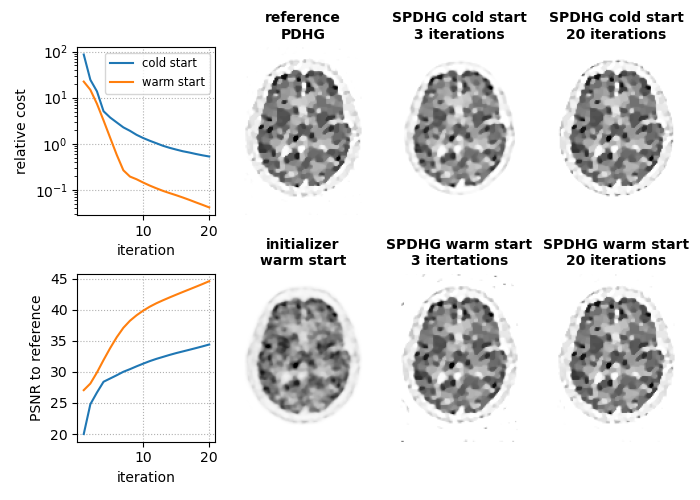
\includegraphics[width=1.0\columnwidth]{figs/SPDHG_cold_vs_warm_start.png}
  \caption{Comparison of convergence of sinogram SPDHG using a cold and warm start
           for 3e5 counts and a TV prior with $\beta = 0.03$ using 112 subsets.
           For the warm start, $x^0$ was taken from 1 EM-TV iteration with 28 subsets
           and $y^0$ was calculated according to \eqref{eq:yinit}.
           Left column: relative cost and PSNR to with respect to the reference solution as
           a function of the iterations.
           Second column: reference PDHG reconstruction using 20000 iterations (top) and
           initializer $x^0$ used in the warm start.
           Third column: Reconstructions after 3 iterations with cold start (top) and warm
           start (bottom).
           Fourth column: Reconstructions after 20 iterations.
           Note that in the calculation of the relative cost the same $x^0$ was used
           and that in both cases the same step size ratio $\gamma$ was used.
          }
  \label{fig:warm_start}
\end{figure}

%include all figures already here to distribute them better over the text
\begin{figure*}
  \centering
  \begin{subfigure}[]{1.0\textwidth}
    \centering
    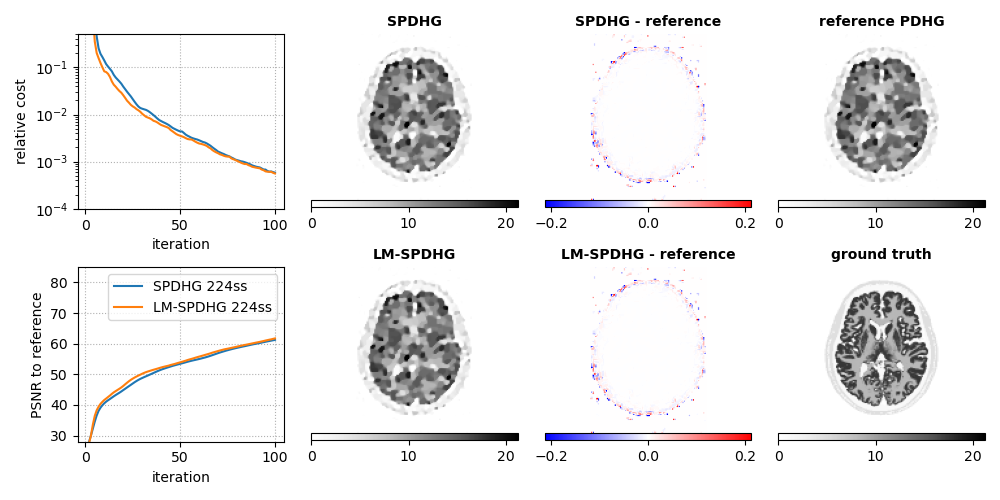
\includegraphics[width=0.8\textwidth]{./figs/brain2d_counts_3.0E+05_seed_1_beta_3.0E-02_prior_TV_niter_ref_20000_fwhm_4.5_4.5_niter_100.png}
    \caption{3e5 true (5e5 prompt) counts, TV prior, $\beta = 0.03$}
  \end{subfigure}
  \vfill
  \begin{subfigure}[]{1.0\textwidth}
    \centering
    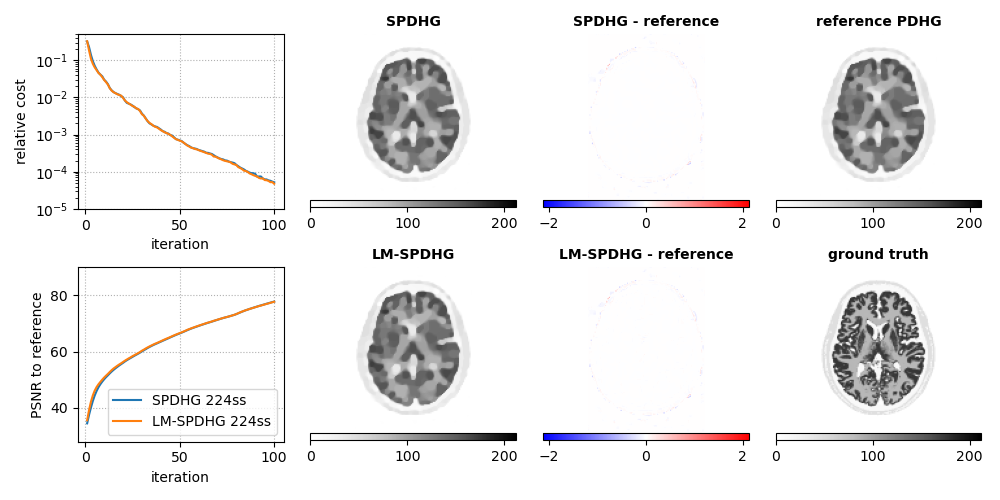
\includegraphics[width=0.8\textwidth]{./figs/brain2d_counts_3.0E+06_seed_1_beta_3.0E-02_prior_TV_niter_ref_20000_fwhm_4.5_4.5_niter_100.png}
    \caption{3e6 true (5e6 prompt) counts, TV prior, $\beta = 0.03$}
  \end{subfigure}
  \vfill
  \begin{subfigure}[]{1.0\textwidth}
    \centering
    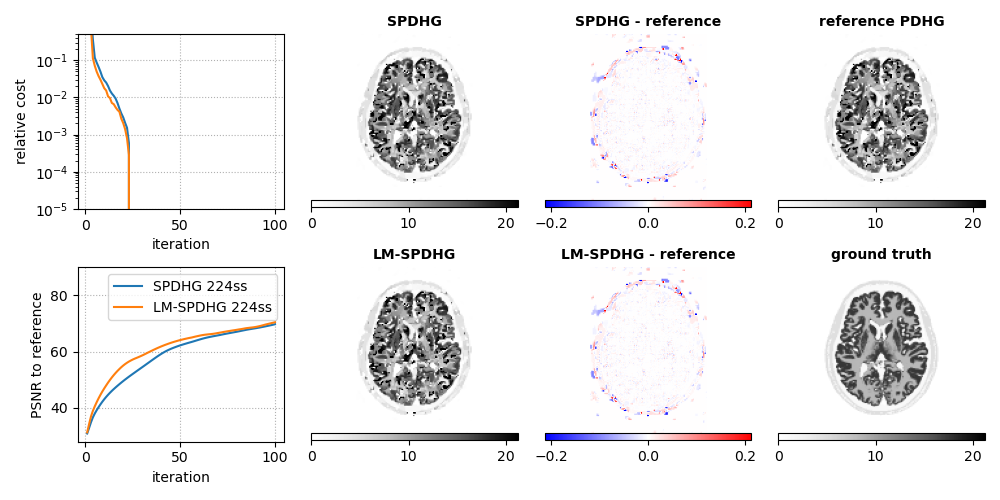
\includegraphics[width=0.8\textwidth]{./figs/brain2d_counts_3.0E+05_seed_1_beta_1.0E-01_prior_DTV_niter_ref_20000_fwhm_4.5_4.5_niter_100.png}
    \caption{3e5 true (5e5 prompt) counts, DTV prior, $\beta = 0.1$}
  \end{subfigure}
  \caption{Comparison of convergence of sinogram SPDHG and LM-SPDHG
           for using 244 subsets.
           All three subfigures (a) - (c) show the same quantities but for
           different count levels and priors.
           Left column: relative cost and PSNR to with respect to the reference solution as
           a function of the iterations for sinogram SPDHG (blue) and LM-SPDHG (orange).
           Second column: SPDHG (top) and LM-SPDHG (bottom) reconstruction after 100 iterations.
           Third column: absolute difference between SPDHG/LM-SPDHG and reference PDHG reconstruction.
           Forth column: reference PDHG reconstruction using 20000 iterations (top) and ground truth
           used to generate the data (bottom).}
  \label{fig:lm-spdhg-var}
\end{figure*}

\begin{figure*}
  \centering
  \begin{subfigure}[]{1.0\textwidth}
    \centering
    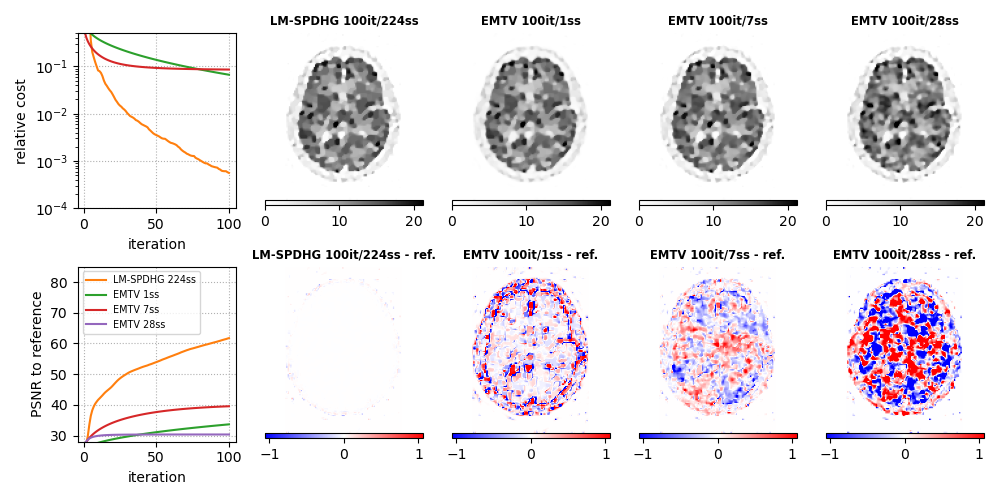
\includegraphics[width=0.8\textwidth]{./figs/brain2d_counts_3.0E+05_seed_1_beta_3.0E-02_prior_TV_niter_ref_20000_fwhm_4.5_4.5_niter_100_emtv.png}
    \caption{3e5 true (5e5 prompt) counts, TV prior, $\beta = 0.03$}
  \end{subfigure}
  \vfill
  \begin{subfigure}[]{1.0\textwidth}
    \centering
    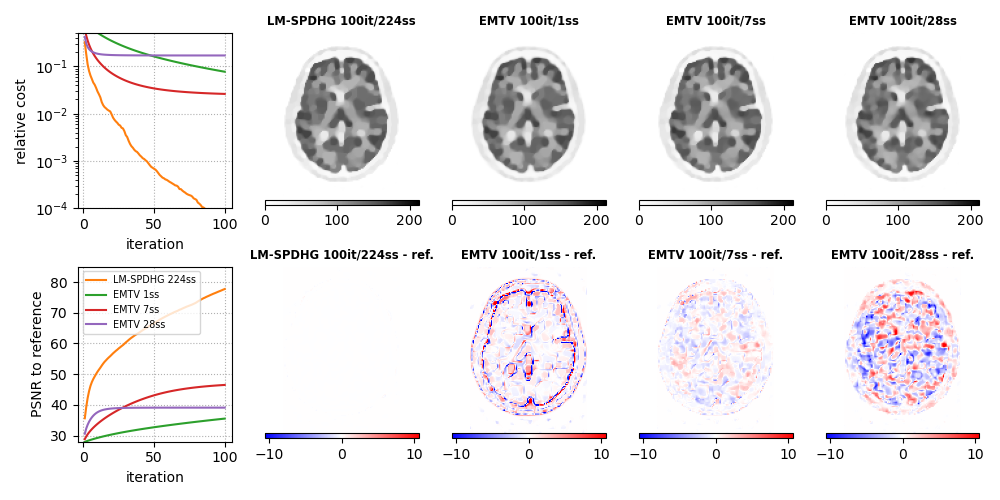
\includegraphics[width=0.8\textwidth]{./figs/brain2d_counts_3.0E+06_seed_1_beta_3.0E-02_prior_TV_niter_ref_20000_fwhm_4.5_4.5_niter_100_emtv.png}
    \caption{3e6 true (5e6 prompt) counts, TV prior, $\beta = 0.03$}
  \end{subfigure}
  \vfill
  \begin{subfigure}[]{1.0\textwidth}
    \centering
    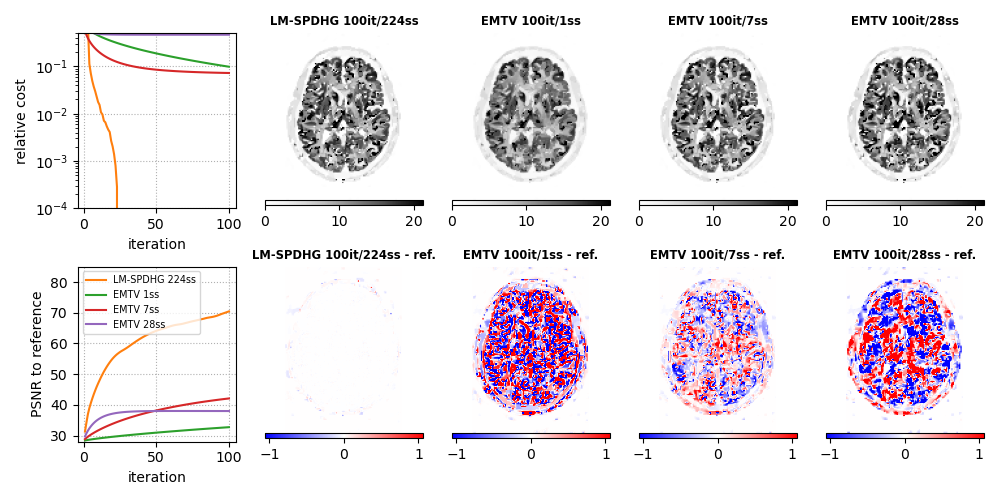
\includegraphics[width=0.8\textwidth]{./figs/brain2d_counts_3.0E+05_seed_1_beta_1.0E-01_prior_DTV_niter_ref_20000_fwhm_4.5_4.5_niter_100_emtv.png}
    \caption{3e5 true (5e5 prompt) counts, DTV prior, $\beta = 0.1$}
  \end{subfigure}
  \caption{Same as Fig.~\ref{fig:lm-spdhg-var} but comparing the convergence of LM-SPDHG using
           224 subsets and listmode EM-TV using 1, 7 and 28 subsets.
           The top row of images shows the reconstruction after 100 iterations and the bottom
           row shows the difference to the reference reconstruction which is shown in
           Fig.~\ref{fig:lm-spdhg-var}.
           Note that the width of the color window in the difference plots is five times wider
           compared to Fig.~\ref{fig:lm-spdhg-var}.}
  \label{fig:emtv}
\end{figure*}


\begin{figure*}
  \centering
  \begin{subfigure}[b]{0.23\textwidth}
    \centering
    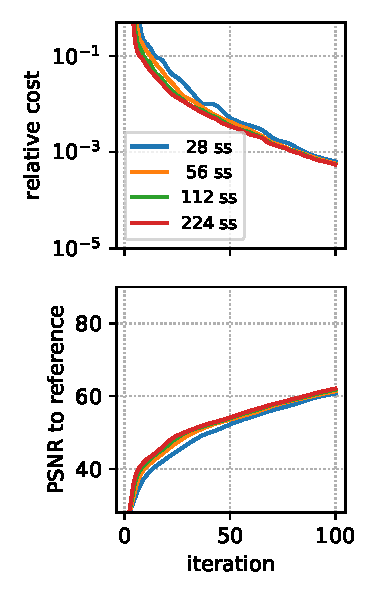
\includegraphics[width=1.0\textwidth]{./figs/brain2d_counts_3.0E+05_seed_1_beta_3.0E-02_prior_TV_niter_ref_20000_fwhm_4.5_4.5_niter_100_ss.pdf}
    \caption{3e5 true (5e5 prompt) counts, TV prior, $\beta = 0.03$}
  \end{subfigure}
  \hfill
  \begin{subfigure}[b]{0.23\textwidth}
    \centering
    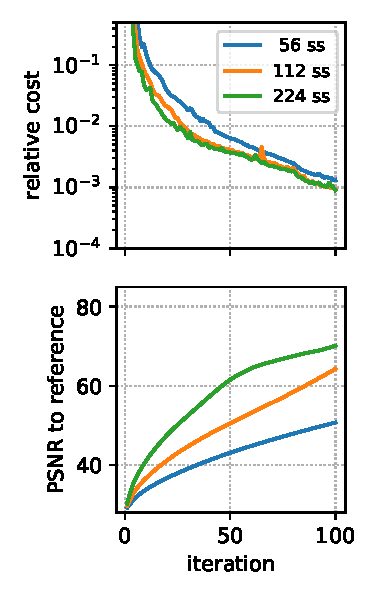
\includegraphics[width=1.0\textwidth]{./figs/brain2d_counts_3.0E+05_seed_1_beta_1.0E-01_prior_DTV_niter_ref_20000_fwhm_4.5_4.5_niter_100_ss.pdf}
    \caption{3e5 true (5e5 prompt) counts, DTV prior, $\beta = 0.1$}
  \end{subfigure}
  \hfill
  \begin{subfigure}[b]{0.23\textwidth}
    \centering
    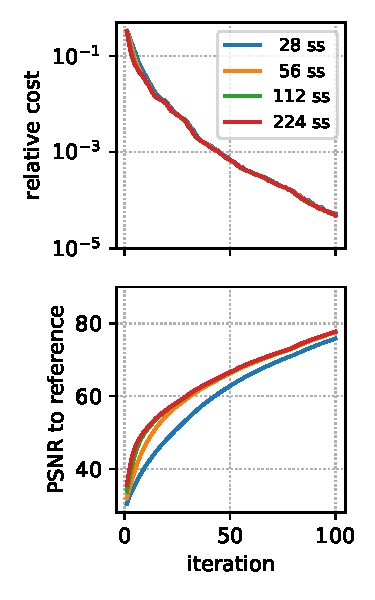
\includegraphics[width=1.0\textwidth]{./figs/brain2d_counts_3.0E+06_seed_1_beta_3.0E-02_prior_TV_niter_ref_20000_fwhm_4.5_4.5_niter_100_ss.pdf}
    \caption{3e6 true (5e5 prompt) counts, TV prior, $\beta = 0.03$}
  \end{subfigure}
  \hfill
  \begin{subfigure}[b]{0.23\textwidth}
    \centering
    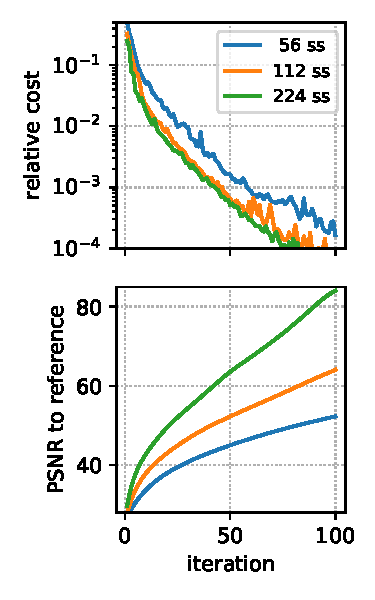
\includegraphics[width=1.0\textwidth]{./figs/brain2d_counts_3.0E+06_seed_1_beta_1.0E-01_prior_DTV_niter_ref_20000_fwhm_4.5_4.5_niter_100_ss.pdf}
    \caption{3e6 true (5e5 prompt) counts, DTV prior, $\beta = 0.1$}
  \end{subfigure}

  \caption{Converge of LM-SPDHG for different number of subsets at two count levels for the TV and 
           DTV prior. Note that when increasing the number of data subsets, the number of gradient
           updates per iteration increases as well.}
  \label{fig:num_subsets}
\end{figure*}

\begin{figure*}
  \centering
    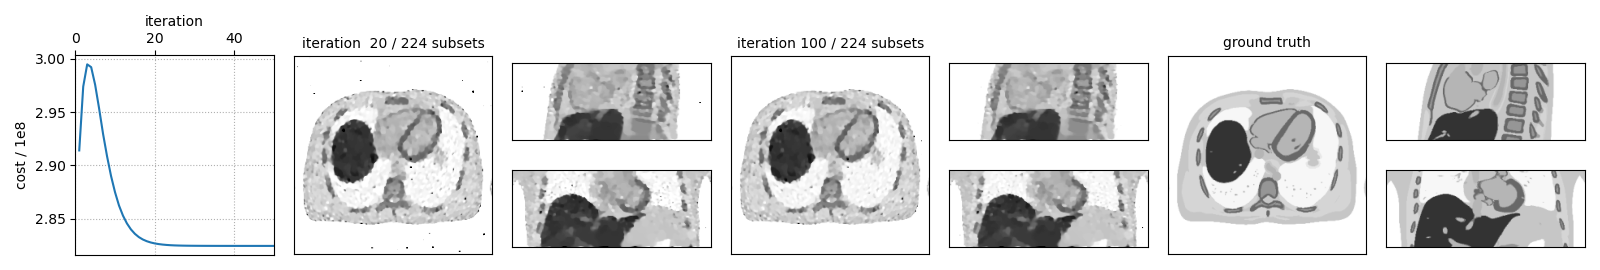
\includegraphics[width=1.0\textwidth]{./figs/xcat_TV_3e-2_4e7.png}
  \caption{Convergence of LM-SPDHG for reconstruction of 3D TOF data generated from the XCAT phantom
           using 4e7 true (7e7) prompt counts and a TV prior with $\beta = 0.03$.
           Left column: evolution of cost function. 
           Columns 2-3: transversal, sagittal and coronal
           slice of LM-SPDHG reconstruction after 20 iterations and 224 subsets.
           Columns 4-5: LM-SPDHG reconstruction after 100 iterations and 224 subsets.
           Columns 6-7: Ground truth image.}
  \label{fig:xcat}
\end{figure*}


Recalling the fact that for most common TOF PET acquisitions, LM-SPDHG requires less memory and 
is also faster, one would probably prefer LM-SPDHG over SPDHG if the speed of convergence is the same.
In the following, we describe a set of numerical experiments that we conducted to show that this
is indeed the case.
In the absence of an analytical solution to the optimization problems \eqref{eq:primal}
and \eqref{eq:saddle}, we analyzed the convergence of LM-SPDHG and SPDHG with respect to a 
reference solution $x^*$ as done in \cite{Ehrhardt2019}.
Convergence was monitored by tracking the relative cost function
\begin{equation}
c_\text{rel}(x) = (c(x) - c(x^*)) / (c(x^0) - c(x^*)) \ ,
\end{equation}
where $c(x)$ is the cost function to be optimized in \eqref{eq:primal} and $x^0$ is the initial value
used for $x$.
Moreover, convergence was also montiored in image space by tracking the peak signal-to-noise ratio
with respect to $x^*$
\begin{equation}
\text{PSNR}(x) = 20\,\log_{10} \left( \|x^*\|_\infty/\sqrt{\text{MSE}(x,x^*)} \right) \ ,
\end{equation}
where MSE is the mean squared error.
The reference solution was obtained by running the deterministic PDHG (SPDHG without subsets)
for 20000 iterations.
Since running PDHG with 20000 iterations using realistic 3D TOF PET data takes a very long 
time (approx. 250\,h), all numerical convergence experiments were performed using simulated 2D TOF PET data.
A 2D software brain phantom with a gray to white matter contrast of 4:1 was created
based on the brainweb phantom \cite{Collins1998} and used to generate simulated 2D TOF data 
including the effects of limited spatial resolution, attenuation and a flat contamination mimicking 
random and scattered coincidences with a contamination fraction of 42\%.
The geometry and TOF resolution of the simulated 2D PET system was chosen to 
mimic one direct plane of a state-of-the art TOF PET scanner with a ring diameter of 650\,mm
and a 400\,ps TOF resolution
(sinogram dimension: 357 radial bins, 224 projection angles, 27 TOF bins).
Noisy simulated prompt emission TOF sinograms and corresponding listmode data were generated
for two different count levels (5e5 and 5e6 prompt counts).

\begin{algorithm}[t]
\begin{algorithmic}[1]
\small
\State \textbf{Input} event list $N$, contamination list $s_N$
\State \textbf{Split} lists $N$ and $s_N$ into $n$ sublists $N_i$, and $s_{N_i}$
\State \textbf{Pre-compute} sensitivity image $g = P^T 1$
\Repeat
	\State Select subset $i$
	\State $z \gets \dfrac{x\,n}{g} {P_{N_i}^{LM}}^T \dfrac{1}{P_{N_i}^{LM} + s_{N_i}}$ (subset EM step)
  \State $w \gets g / (\beta x)$
  \State $x^+ \gets \argmin_{u\geq 0} \sum_j \dfrac{w_j}{2} \left(u_j -z_j \right)^2 + R(Ku)$
\Until{stopping criterion fulfilled}
\State \Return{$x$}
%\EndFunction
\end{algorithmic}
\caption{listmode EM-TV for PET reconstruction \cite{Sawatzky2008, Burger2008}}
\label{alg:emtv}
\end{algorithm}

Unless stated otherwise, we always applied the EM-TV algorithm, summarized in Algorithm~\ref{alg:emtv}, 
using 1 iteration and 28 subsets to initialize $x^0$ and $y^0$ according to \eqref{eq:yinit}.
To solve the weighted denoising problem in step 8 of the EM-TV algorithm, we applied the
accelerated PDHG algorithm \cite{Chambolle2011} using 20 iterations.

In all SPDHG and LM-SPDHG reconstructios, the step size ratio $\gamma$ was set 
to $3 / \|x^0\|_\infty$ and $\rho$ was set to 0.999.
When splitting the data into $n$ subsets, the vector of probabilities determining 
whether an update with respect to a subset of the data or with respect to the prior is 
done was set to 
%
\begin{equation}
p_k = 
  \begin{cases}
  \frac{1}{2n} \ &\text{if } k \leq n \\
  \frac{1}{2}  \ &\text{else} \ ,
  \end{cases}
\end{equation}
%
such that on average an update with respect to the prior was done on every second update
as suggested in \cite{Ehrhardt2019}. 
In this work, we use the term iteration for $2n$ updates such that on average in every iteration
the complete data is forward and backprojected once and $n$ updates with respect to the
prior are performed.

As benchmark examples for non-smooth priors, we consider two ``Total Variation like'' priors
in this work. 
These priors have the form
%
\begin{equation}
  R(Kx) = \|K x\|_{2,1} \ ,
\end{equation}
%
where $\|K x \|_{2,1}$ is the sum over all entries of the pointwise Euclidean norm of $K x$
(mixed L2-L1 norm).
The proximal operator for the convex dual of this prior is given by
%
\begin{equation}
(\prox_{R^*}^S(w) )_i = \frac{w_i}{\max(1,|w_i|)} \ .
\end{equation}
%
For the linear operator $K$, we first used the finite forward difference operator resulting
in the classical Total Variation (TV) prior \cite{Rudin1992}.
Moreover, we also implemented the Directional Total Variation (DTV) prior incorporating
structural information by only considering the component of the finite difference vector 
that is perpendicular to a joint gradient field in every point \cite{Ehrhardt2016}.
In our convergence experiments using DTV, we assumed perfect structural prior information
meaning that the joint gradient field used for DTV, was calculated on the ground truth image
itself.
Note that in real acquisitions the quality of the available structural prior information is
of course inferior. 
However, we do not expect that this fact strongly affects the convergence properties of 
SPDHG and LM-SPDHG. 

To demonstrate that LM-SPDHG also works for realistic 3D TOF listmode data,
we finally simulated and reconstructed 3D TOF PET data based on the 3D XCAT \cite{Segars2010} phantom 
and a state-of-the-art
TOF PET scanner with 20\,cm axial field of view, a ring diameter of 650\,mm and a 400\,ps TOF 
resolution (sinogram dimension: 357 radial bins, 224 projection angles, 1296 planes, 27 TOF bins).
As before, the data simulation included the effects of attenuation, finite resolution and a
flat contamination with a contamination fraction of 42\%.
In total, 7e7 prompt counts were simulated corresponding approximately to a standard 
80\,s 1\,h p.i. FDG liver bed position acquisition.
Simulated listmode data were reconstructed using LM-SPDHG with 100 iterations and 224 subsets. 

\subsection*{SPDHG using a warm start vs a cold start}

Before investigating the convergence behavior of LM-SPDHG, we first tested whether 
a warm start could already help to lead to faster convergence of SPDHG using sinograms.
Figure~\ref{fig:warm_start} shows the results of SPDHG reconstructions with a cold 
($x^0 = 0$ and $y^0 = 0$) and warm start as described above for a data set with 3e5 true counts
and a TV prior with $\beta = 0.03$.
It can be seen that SPDHG with the warm start performs better in terms of relative cost
and PSNR with respect to the reference reconstruction.
A similar trend was observed for higher count levels, with different $\beta$ values and using
the DTV prior indicating that as expected the warm start helps to accelerate convergence
in the early iterations.

\subsection*{Convergence of LM-SPDHG compared to SPDHG}

Figure~\ref{fig:lm-spdhg-var} summarizes the convergence comparison between sinogram SPDHG and 
LM-SPDHG for the same data set and prior as described in the previous subsection using the 
same warm start for both algorithms.
As demonstrated by the convergence metrics and the reconstructed images, the convergence of
sinogram SPDHG and LM-SPDHG is almost identical.
This also holds for different count levels and for the structural DTV priors 
as shown in subfigures (b) and (c) and for different levels of regularization as shown
in supplementary Figs.~1 and 2.
For the example with the DTV prior shown in subfigure (c), the convergence in terms of
PSNR seems to be even slightly faster with LM-SPDHG, which can be also
seen in the difference images with respect to the reference reconstruction.

\subsection*{Convergence of LM-SPDHG compared to listmode EM-TV}

A comparison between the convergence of LM-SPDHG using 224 subsets and listmode 
EM-TV using 1, 7 and 28 subsets is shown in Fig.~\ref{fig:emtv}.
In all sub figures, LM-SPDHG converges much faster than EM-TV.
Interestingly, when using listmode EM-TV with more than one subset, the convergence
metrics saturate meaning that the algorithm probably is stuck
on a limited cycle and the optimal solution is not reached.
When using one subset, the convergence of EM-TV is much slower but does not seem
to saturate after 100 iterations.


\subsection*{Convergence vs number of subsets}

Figure~\ref{fig:num_subsets} shows the convergence of LM-SPDHG as a function of the number of data
subsets used for low (3e5) and high (3e6) counts and the TV and DTV prior.
In general, using 224 subsets leads to faster convergence compared to 56 and 112 subsets.
However, for the TV prior, especially at low counts, there is almost no difference between using
56, 112, and 224 subsets.
In contrast, for the DTV prior, the difference between using 56, 112, and 224 subsets is more
pronounced.
For a fixed number of subsets, convergence is faster for high count compared to low count data sets.


\subsection*{Reconstrution of 3D XCAT data}

Figure~\ref{fig:xcat} shows the results of the reconstruction of the listmode data simulated
from the 3D XCAT phantom using a TV prior with $\beta = 0.03$. 
From the plot of the cost function and the reconstructions shown in the middle, we can see
that reasonable convergence is reached after approximately 25 iterations with 224 subsets.
Note that in contrast to our 2D experiments, the cost function in the first 3 iterations after
the warm start slightly increases before it decreases and stabilizes after around 25 iterations.
As mentioned above, calculating the projections in listmode for 7e7 counts is roughly a factor
of 3 faster compared to sinogram-based processing which substantially speeds up every iteration.
Note that in our proof-of-concept implementation, the effective speed up is less than a 
factor of 3 since we did not implement the gradient operators and proximal mappings on a GPU yet
which leads to overhead due to gradient-based updates.
However, we expect that, once properly implemented on GPUs, this overhead will be small compared to
the time needed to calculate the actual TOF projections.


%%%%%%%%%%%%%%%%%%%%%%%%%%%%%%%%%%%%%%%%%%%%%%%%%%%%%%%%%%%%%%%%%%%%%%%%%%%%%%%%%%%%%%%%%%%%%%%%%%%%%%%%

\section{Discussion}

The results of our numerical experiments presented in this work demonstrate that the speed of 
convergence of LM-SPDHG is essentially the same as the one of the original SPDHG using
sinograms.
For almost all clinical acquisitions with state-of-the-art TOF PET scanners resulting in extremely
sparse data, LM-SPDHG has two distinct advantages compared to SPDHG.
First, during the iterations all forward and back projections can be performed in listmode
which is faster compared to sinogram projectors for sparse TOF data.

Second, as shown in Table~\ref{tab:mem}, the memory requirements are substantially reduced such
that even for an aquisition with 5e8 prompt coincidences only 12.5\,GB of memory are needed.
This actually enables a pure GPU-implementation on of LM-SPDHG avoiding intermediate memory
transfer between the host and a state-of-the-art GPU with a memory of approximately 16\,GB.
Note that in our proof of concept implementation of LM-SPDHG we used a hybrid computing
approach where only the TOF PET forward and back projections where computed using a GPU.
We expect that once properly implemented purely on a GPU, the computation time required
for LM-SPDHG will further decrease since memory transfter between host and GPU is a bottleneck 
in our implementation.
Note that a pure GPU implementation of the conventional SPDHG algorithm for modern TOF PET
data is more complicated since more than 50\,GB of GPU is required.

In this proof of concept work, we only used two non-smooth TV-like priors
to benchmark LM-SPDHG. 
Note that in general, SPDHG and LM-SPDHG can be also used for smooth priors as long
as proximal operator of the convex dual of the prior can be efficiently calculated which is
e.g. the case for prior penalizing the squared L2 norm or Huber TV.
However, for smooth priors the speed of convergence of (LM)-SPDHG should be benchmarked against
other stochastic gradient-based optimization techniques such as the stochastic variance reduced gradient (SVRG) \cite{Johnson2013} or SAGA \cite{Defazio2014} which is beyond the scope of this work.
We also note that in this work we a used scalar spatially-invariant prior strength $\beta$ which
leads to a spatially-variant local pertubation response (LPR). 
For pratical applications where a spatially-invariant is desirable, a spatially-varient prior 
strength should be used as described in \cite{Ahn2008,Tsai2020}.

Last but not least, we would like to emphasize that the listmode EM-TV algorithm
is still a very practical and useful algorithm to approximate the solution 
of the optimization problem \eqref{eq:primal} for listmode data and non-smooth priors.
However, as shown in Fig.~\ref{fig:emtv}, it seems that when using ordered subsets for acceleration,
EM-TV does not reach the optimal solution but rather remains on a limit cycle similar to the
behaviour of OSEM.
Whether the difference between the limit cycle and the true optimal solution is of importance
for a given count level and clinical task, should be investigated in the future.


\printbibliography


%\section{Introduction}
%\label{sec:introduction}
%\IEEEPARstart{T}{his} document is a template for \LaTeX.
%You are encouraged to use it to prepare your manuscript.
%If you are reading a paper or PDF version of this document, please download the 
%\LaTeX .zip file from the IEEE Web site at \underline
%{https://www.embs.org/tmi/authors-instructions/} to prepare your manuscript.
%You can also explore using the Overleaf editor at 
%\underline
%{https://www.overleaf.com/blog/278-how-to-use-overleaf-with-}\discretionary{}{}{}\underline
%{ieee-collabratec-your-quick-guide-to-getting-started\#.}\discretionary{}{}{}\underline{xsVp6tpPkrKM9}
%
%\section{Guidelines for Manuscript Preparation}
%Do not change the template font sizes or line spacing to squeeze more text into a limited number of pages.
%The preferred font is 10-pt Times New Roman. Use italics for emphasis; do not underline words.
%
%Place your figures in the text as you expect them to appear in print. Further instructions
%on figure usage appear in Section VI. Although IEEE will do the final formatting of your paper,
%we expect you to approximate the final form appearance for all versions
%submitted to TMI via ScholarOne\textregistered to the extent possible.
%
%\subsection{Abbreviations and Acronyms}
%Define abbreviations and acronyms the first time they are used in the text, 
%even after they have already been defined in the abstract. Abbreviations 
%such as IEEE, SI, ac, and dc do not have to be defined. Abbreviations that 
%incorporate periods should not have spaces: write ``C.N.R.S.,'' not ``C. N. 
%R. S.'' Do not use abbreviations in the title unless they are unavoidable 
%(for example, ``IEEE'' in the title of this article).
%
%\subsection{Other Recommendations}
%Use one space after periods and colons. Hyphenate complex modifiers: 
%``zero-field-cooled magnetization.'' Avoid dangling participles, such as, 
%``Using \eqref{eq}, the potential was calculated.'' It is not clear who or what 
%used \eqref{eq}. Write instead, ``The potential was calculated by using \eqref{eq},'' or 
%``Using \eqref{eq}, we calculated the potential.''
%
%Use a zero before decimal points: ``0.25,'' not ``.25.'' Use 
%``cm$^{3}$,'' not ``cc.'' Indicate sample dimensions as ``0.1 cm 
%$\times $ 0.2 cm,'' not ``0.1 $\times $ 0.2 cm$^{2}$.'' The 
%abbreviation for ``seconds'' is ``s,'' not ``sec.'' Use 
%``Wb/m$^{2}$'' or ``webers per square meter,'' not 
%``webers/m$^{2}$.'' When expressing a range of values, write ``7 to 
%9'' or ``7--9,'' not ``7$\sim $9.''
%
%A parenthetical statement at the end of a sentence is punctuated outside of 
%the closing parenthesis (like this). (A parenthetical sentence is punctuated 
%within the parentheses.) In American English, periods and commas are located within 
%quotation marks, like ``this period.'' Other punctuation is placed ``outside''! 
%Avoid contractions; for example, write ``do not'' instead of ``don't.'' The 
%serial comma is preferred: ``A, B, and C'' instead of ``A, B and C.''
%
%If you wish, you may write in the first person singular or plural form using
%the active voice (``I observed that $\ldots$'' or ``We observed that $\ldots$'' 
%instead of ``It was observed that $\ldots$''). Remember to check spelling. If 
%your native language is not English, please have a native English-speaking 
%colleague to carefully proofread your paper.
%
%\section{Math}
%\subsection{Equations}
%Number equations consecutively with equation numbers in parentheses flush 
%with the right margin, as appears in \eqref{eq}. Refer to ``\eqref{eq},'' not ``Eq. \eqref{eq}'' 
%or ``equation \eqref{eq},'' except at the beginning of a sentence: ``Equation \eqref{eq} 
%is $\ldots$ .'' To make your equations more 
%compact, you may use the solidus (~/~), the exp function, or appropriate 
%exponents. Use parentheses to avoid ambiguities in denominators. Punctuate 
%equations when they are part of a sentence, as in
%\begin{equation}E=mc^2.\label{eq}\end{equation}
%
%Be sure to define the symbols in your equation before the equation appears or
%immediately following. Italicize symbols ($T$ might refer 
%to temperature, but T is the unit tesla).
%
%\subsection{\LaTeX-Specific Advice}
%
%Use ``soft'' (e.g., \verb|\eqref{Eq}|) cross references instead
%of ``hard'' references (e.g., \verb|(1)|). This will make it possible
%to combine sections, add equations, or change the order of figures or
%citations without having to manually change equation references.
%
%Do not use the \verb|{eqnarray}| equation environment. Use
%\verb|{align}| or \verb|{IEEEeqnarray}| instead. The \verb|{eqnarray}|
%environment leaves unsightly spaces around relation symbols.
%
%Note that the \verb|{subequations}| environment in {\LaTeX}
%will increment the main equation counter even when there are no
%equation numbers displayed.
%
%{\BibTeX} only functions in conjunction with local .bib files. If you use {\BibTeX} to produce the
%bibliography you must attach the .bib files.
%
%{\LaTeX} can't read your mind. If you assign the same label to both a
%subsubsection and a table, you may find that Table I has been cross
%referenced as Table IV-B3. 
%
%{\LaTeX} does not have precognitive abilities. If you put a
%\verb|\label| command before the command that updates the counter it's
%supposed to be using, the label will pick up the last counter to be
%cross referenced instead. In particular, a \verb|\label| command
%should not go before the caption of a figure or a table.
%
%Do not use \verb|\nonumber| inside the \verb|{array}| environment. It
%will not stop equation numbers inside \verb|{array}| and it might stop a
%wanted equation number in the surrounding equation.
%
%If you are submitting your paper to a colorized journal, you can use
%the following two lines at the start of the article to ensure its
%appearance resembles the final copy:
%
%\smallskip\noindent
%\begin{small}
%\begin{tabular}{l}
%\verb+\+\texttt{documentclass[journal,twoside,web]\{ieeecolor\}}\\
%\verb+\+\texttt{usepackage\{\textit{Journal\_Name}\}}
%\end{tabular}
%\end{small}
%
%\section{Units}
%Use either SI (MKS) or CGS as primary units. (SI units are strongly 
%encouraged.) English units may be used as secondary units (in parentheses). 
%For example, write ``1 kg (2.2lb).'' An exception exists for when 
%English units are used as identifiers in commercial products, such as a ``3\textonehalf-in 
%disk drive.'' Avoid combining SI and CGS units, such as current in amperes 
%and magnetic field in oersteds. This often leads to confusion because 
%equations do not balance dimensionally. If you must use mixed units, clearly 
%state the units for each quantity in an equation.
%
%The SI unit for magnetic field strength $H$ is A/m. However, if you wish to use 
%units of T, either refer to magnetic flux density $B$ or magnetic field 
%strength symbolized as $\mu _{0}H$. Use the center dot to separate 
%compound units, e.g., ``A$\cdot $m$^{2}$.''
%
%\begin{figure}[!t]
%\centerline{\includegraphics[width=\columnwidth]{fig1.png}}
%\caption{Magnetization as a function of applied field.
%It is good practice to explain the significance of the figure in the caption.}
%\label{fig1}
%\end{figure}
%
%\section{Guidelines for Graphics Preparation and Submission}
%\label{sec:guidelines}
%
%\subsection{Types of Graphics}
%The following list outlines the different types of graphics published in 
%IEEE journals. They are categorized based on their construction, and use of 
%color~/~shades of gray:
%
%\subsubsection{Color/Grayscale figures}
%{Figures that are meant to appear in color, or shades of black/gray. Such 
%figures may include photographs, illustrations, multicolor graphs, and 
%flowcharts.}
%
%\subsubsection{Line Art figures}
%{Figures that are composed of only black lines and shapes. These figures 
%should have no shades or half-tones of gray, only black and white.}
%
%\subsubsection{Author photos}
%{Not allowed for papers in TMI.}
%
%\subsubsection{Tables}
%{Data charts which are typically black and white, but sometimes include 
%color.}
%
%\begin{table}
%\caption{Units for Magnetic Properties}
%\label{table}
%\setlength{\tabcolsep}{3pt}
%\begin{tabular}{|p{25pt}|p{75pt}|p{115pt}|}
%\hline
%Symbol& 
%Quantity& 
%Conversion from Gaussian and \par CGS EMU to SI $^{\mathrm{a}}$ \\
%\hline
%$\Phi $& 
%magnetic flux& 
%1 Mx $\to  10^{-8}$ Wb $= 10^{-8}$ V$\cdot $s \\
%$B$& 
%magnetic flux density, \par magnetic induction& 
%1 G $\to  10^{-4}$ T $= 10^{-4}$ Wb/m$^{2}$ \\
%$H$& 
%magnetic field strength& 
%1 Oe $\to  10^{3}/(4\pi )$ A/m \\
%$m$& 
%magnetic moment& 
%1 erg/G $=$ 1 emu \par $\to 10^{-3}$ A$\cdot $m$^{2} = 10^{-3}$ J/T \\
%$M$& 
%magnetization& 
%1 erg/(G$\cdot $cm$^{3}) =$ 1 emu/cm$^{3}$ \par $\to 10^{3}$ A/m \\
%4$\pi M$& 
%magnetization& 
%1 G $\to  10^{3}/(4\pi )$ A/m \\
%$\sigma $& 
%specific magnetization& 
%1 erg/(G$\cdot $g) $=$ 1 emu/g $\to $ 1 A$\cdot $m$^{2}$/kg \\
%$j$& 
%magnetic dipole \par moment& 
%1 erg/G $=$ 1 emu \par $\to 4\pi \times  10^{-10}$ Wb$\cdot $m \\
%$J$& 
%magnetic polarization& 
%1 erg/(G$\cdot $cm$^{3}) =$ 1 emu/cm$^{3}$ \par $\to 4\pi \times  10^{-4}$ T \\
%$\chi , \kappa $& 
%susceptibility& 
%1 $\to  4\pi $ \\
%$\chi_{\rho }$& 
%mass susceptibility& 
%1 cm$^{3}$/g $\to  4\pi \times  10^{-3}$ m$^{3}$/kg \\
%$\mu $& 
%permeability& 
%1 $\to  4\pi \times  10^{-7}$ H/m \par $= 4\pi \times  10^{-7}$ Wb/(A$\cdot $m) \\
%$\mu_{r}$& 
%relative permeability& 
%$\mu \to \mu_{r}$ \\
%$w, W$& 
%energy density& 
%1 erg/cm$^{3} \to  10^{-1}$ J/m$^{3}$ \\
%$N, D$& 
%demagnetizing factor& 
%1 $\to  1/(4\pi )$ \\
%\hline
%\multicolumn{3}{p{251pt}}{Vertical lines are optional in tables. Statements that serve as captions for 
%the entire table do not need footnote letters. }\\
%\multicolumn{3}{p{251pt}}{$^{\mathrm{a}}$Gaussian units are the same as cg emu for magnetostatics; Mx 
%$=$ maxwell, G $=$ gauss, Oe $=$ oersted; Wb $=$ weber, V $=$ volt, s $=$ 
%second, T $=$ tesla, m $=$ meter, A $=$ ampere, J $=$ joule, kg $=$ 
%kilogram, H $=$ henry.}
%\end{tabular}
%\label{tab1}
%\end{table}
%
%\subsection{Multipart figures}
%Multipart figures are comprised of more than one sub-figure presented together.
%If a multipart figure is made up of multiple figure types (one part is lineart,
%and another is grayscale or color) the figure should meet the strictest applicable guidelines.
%
%\subsection{File Formats For Graphics}
%\label{formats}
%Format and save your graphics as one of the following approved file types:
%PostScript (.PS), Encapsulated PostScript (.EPS), Tagged Image File Format (.TIFF),
%Portable Document Format (.PDF), Portable Network Graphics (.PNG), or Metapost (.MPS).
%After the paper is accepted, any included graphics must be submitted alongside the final manuscript files.
%
%\subsection{Sizing of Graphics}
%Most charts, graphs, and tables are one column wide (3.5 inches~/~88 
%millimeters) or page wide (7.16 inches~/~181 millimeters). The maximum
%depth of a graphic is 8.5 inches (216 millimeters). When choosing the depth of a graphic,
%please allow space for a caption. Authors are allowed to size figures between column and
%page widths, but it is recommended not to size figures less than column width unless necessary. 
%
%\subsection{Resolution}
%The proper resolution of your figures will depend on the type of figure it 
%is as defined in the ``Types of Figures'' section. Author photographs, 
%color, and grayscale figures should be at least 300dpi. Lineart, including 
%tables should be a minimum of 600dpi.
%
%\subsection{Vector Art}
%While IEEE does accept and even recommends that authors submit artwork
%in vector format, it is our policy is to rasterize all figures for publication. This is done
%in order to preserve figures' integrity across multiple computer platforms.
%
%\subsection{Colorspace}
%The term colorspace refers to the entire sum of colors that can be 
%represented within a given medium. For our purposes, the three main colorspaces
%are grayscale, RGB (red/green/blue) and CMYK (cyan/magenta/yellow/black).
%RGB is generally used with on-screen graphics, whereas CMYK is used for printing purposes.
%
%All color figures should be generated in RGB or CMYK colorspace. Grayscale 
%images should be submitted in grayscale colorspace. Line art may be 
%provided in grayscale OR bitmap colorspace. Note that ``bitmap colorspace'' 
%and ``bitmap file format'' are not the same thing. When bitmap colorspace 
%is selected, .TIF/.TIFF are the recommended file formats.
%
%\subsection{Accepted Fonts Within Figures}
%When preparing your graphics IEEE suggests that you use of one of the 
%following Open Type fonts: Times New Roman, Helvetica, Arial, Cambria, and 
%Symbol. If you are supplying EPS, PS, or PDF files all fonts must be 
%embedded. Some fonts may only be native to your operating system; without 
%the fonts embedded, parts of the graphic may be distorted or missing.
%
%A safe option when finalizing your figures is to strip out the fonts before 
%you save the files, creating ``outline'' type. This converts fonts to 
%artwork that will appear uniformly on any screen.
%
%\subsection{Using Labels Within Figures}
%
%\subsubsection{Figure Axis labels}
%Figure axis labels are often a source of confusion. Use words rather than 
%symbols. As an example, write the quantity ``Magnetization,'' or 
%``Magnetization M,'' not just ``M.'' Put units in parentheses. Do not label 
%axes only with units. As in Fig. 1, for example, write ``Magnetization 
%(A/m)'' or ``Magnetization (A$\cdot$m$^{-1}$),'' not just ``A/m.''
%Do not label axes with a ratio of quantities and units.
%For example, write ``Temperature (K),'' not ``Temperature/K.'' 
%
%Multipliers can be especially confusing. Write ``Magnetization (kA/m)'' or 
%``Magnetization (10$^{3}$ A/m).'' Do not write ``Magnetization 
%(A/m)$\,\times\,$1000'' because the reader would not know whether the top 
%axis label in Fig. 1 meant 16000 A/m or 0.016 A/m. Figure labels should be 
%legible, approximately 8 to 10 point type.
%
%\subsubsection{Subfigure Labels in Multipart Figures and Tables}
%Multipart figures should be combined and labeled before final submission. 
%Labels should appear centered below each subfigure in 8 point Times New 
%Roman font in the format of (a) (b) (c).
%
%\subsection{Referencing a Figure or Table Within Your Paper}
%When referencing your figures and tables within your paper, use the 
%abbreviation ``Fig.'' even at the beginning of a sentence. Do not abbreviate 
%``Table.'' Tables should be numbered with Roman numerals.
%
%\subsection{Submitting Your Graphics}
%Format your paper with the graphics included within the body of the text
%as you would expect to see the paper in print. Please do this at each stage of the review,
%from first submission to final files. For final files only, after the paper has been accepted
%for publication, figures should also be submitted individually in addition to the manuscript
%file using one of the approved file formats. Place a figure caption below each figure;
%place table titles above the tables. Do not include captions or borders in the uploaded figure files.
%
%\subsection{File Naming}
%Figures (line artwork or images) should be named starting with the 
%first 5 letters of the corresponding author's last name. The next characters in the 
%filename should be the number that represents the figure's sequential 
%location in the article. For example, in author ``Anderson's'' paper,
%the first three figures might be named ander1.tif, ander2.tif, and ander3.ps.
%
%Tables should contain only the body of the table (not the caption) and 
%should be named similarly to figures, except that `.t' is inserted 
%in-between the author's name and the table number. For example, author 
%Anderson's first three tables would be named ander.t1.tif, ander.t2.ps, ander.t3.eps.
%
%Author photographs or biographies are not permitted in IEEE TMI papers.
%
%\subsection{Checking Your Figures: The IEEE Graphics Analyzer}
%The IEEE Graphics Analyzer enables authors to pre-screen their graphics for 
%compliance with IEEE Transactions and Journals standards before submission. 
%The online tool, located at \underline{http://graphicsqc.ieee.org/},
%allows authors to upload their graphics in order to check that each file is the correct file format,
%resolution, size and colorspace; that no fonts are missing or corrupt;
%that figures are not compiled in layers or have transparency,
%and that they are named according to the IEEE Transactions and Journals naming convention.
%At the end of this automated process, authors are provided with 
%a detailed report on each graphic within the web applet, as well as by email.
%
%For more information on using the Graphics Analyzer or any other graphics 
%related topic, contact the IEEE Graphics Help Desk by e-mail at 
%graphics@ieee.org.
%
%\subsection{Color Processing/Printing in IEEE Journals}
%All IEEE Transactions, Journals, and Letters allow an author to publish 
%color figures on IEEE Xplore\textregistered\ at no charge, and automatically 
%convert them to grayscale for print versions. In most journals, figures and 
%tables may alternatively be printed in color if an author chooses to do so. 
%Please note that this service comes at an extra expense to the author. If 
%you intend to have print color graphics, include a note with your final 
%paper indicating which figures or tables you would like to be handled that way,
%and stating that you are willing to pay the additional fee.
%
%\section{Some Common Mistakes}
%The word ``data'' is plural, not singular. The subscript for the 
%permeability of vacuum $\mu _{0}$ is zero, not a lowercase letter 
%``o.'' Use the word ``micrometer'' instead of ``micron.'' A graph within a graph is an 
%``inset,'' not an ``insert.'' The word ``alternatively'' is preferred to the 
%word ``alternately'' (unless you really mean something that alternates). Use 
%the word ``whereas'' instead of ``while'' (unless you are referring to 
%simultaneous events). Do not use the word ``essentially'' to mean 
%``approximately'' or ``effectively.'' Do not use the word ``issue'' as a 
%euphemism for ``problem.'' When compositions are not specified, separate 
%chemical symbols by en-dashes; for example, ``NiMn'' indicates the 
%intermetallic compound Ni$_{0.5}$Mn$_{0.5}$ whereas 
%``Ni--Mn'' indicates an alloy of some composition 
%Ni$_{x}$Mn$_{1-x}$.
%
%Be aware of the different meanings of the homophones ``affect'' (usually a 
%verb) and ``effect'' (usually a noun), ``complement'' and ``compliment,'' 
%``discreet'' and ``discrete,'' ``principal'' (e.g., ``principal 
%investigator'') and ``principle'' (e.g., ``principle of measurement''). Do 
%not confuse ``imply'' and ``infer.'' 
%
%Prefixes such as ``non,'' ``sub,'' ``micro,'' ``multi,'' and ``ultra'' are 
%not independent words; they should be joined to the words they modify, 
%usually without a hyphen. There is no period after the ``et'' in the Latin 
%abbreviation ``\emph{et al.}'' (it is also italicized). The abbreviation ``i.e.,'' means 
%``that is,'' and the abbreviation ``e.g.,'' means ``for example'' (these 
%abbreviations are not italicized).
%
%A general IEEE styleguide is available at \underline{http://www.ieee.org/web/publications/authors/transjnl/index.ht}
%\discretionary{}{}{}\underline{ml}.
%
%\section{Conclusion}
%A conclusion section is not required. Although a conclusion may review the 
%main points of the paper, do not replicate the abstract as the conclusion.
%A conclusion might elaborate on the importance of the work or suggest 
%applications and extensions.
%
%\appendices
%
%\section*{Appendix and the Use of Supplemental Files}
%Appendices, if needed, appear before the acknowledgment. If an appendix is not
%critical to the main message of the manuscript and is included only for thoroughness
%or for reader reference, then consider submitting appendices as supplemental materials.
%Supplementary files are available to readers through IEEE \emph{Xplore\textregistered}
%at no additional cost to the authors but they do not appear in print versions.
%Supplementary files must be uploaded in ScholarOne as supporting documents, but for
%accepted papers they should be uploaded as Multimedia documents. Refer readers
%to the supplementary files where appropriate within the manuscript text using footnotes.
%\footnote{Supplementary materials are available in the supporting documents/multimedia tab.
%Further instructions on footnote usage are in the Footnotes section on the next page.}
%
%\section*{Acknowledgment}
%The preferred spelling of the word ``acknowledgment'' in American English is 
%without an ``e'' after the ``g.'' Use the singular heading even if you have 
%many acknowledgments. Avoid expressions such as ``One of us (S.B.A.) would 
%like to thank $\ldots$ .'' Instead, write ``F. A. Author thanks $\ldots$ .'' In most 
%cases, sponsor and financial support acknowledgments are placed in the 
%unnumbered footnote on the first page, not here.
%
%\section*{References and Footnotes}
%
%\subsection{References}
%All listed references must be cited in text at least once. Use number citations
%that are placed in square brackets and inside the punctuation.
%
%Multiple references are each numbered with separate brackets.
%When citing a section in a book, please give the relevant page numbers.
%In text, refer simply to the reference number. Do not use ``Ref.'' or
%``reference'' except at the beginning of a sentence:
%``Reference \cite{b3} shows $\ldots$ .'
%
%Reference numbers are set flush left and form a column of their own, hanging 
%out beyond the body of the reference. The reference numbers are on the line, 
%enclosed in square brackets. In all references, the given name of the author 
%or editor is abbreviated to the initial only and precedes the last name.
%List the names of all authors if there are six or fewer co-authors,
%otherwise list the primary author's name followed by \emph{at al.}
%Use commas around Jr., Sr., and III in names. Abbreviate conference titles.
%When citing IEEE transactions, provide the issue number, page range, volume number,
%year, and/or month if available. When referencing a patent, provide the day and 
%month of issue or application. References may not include all information;
%please obtain and include relevant information. Do not combine references.
%There must be only one reference with each number. If there is a 
%URL included with the print reference, it can be included at the end of the reference. 
%
%Other than books, capitalize only the first word in a paper title, except 
%for proper nouns and element symbols. For papers published in translation 
%journals, please give the English citation first, followed by the original 
%foreign-language citation. See the end of this document for formats and 
%examples of common references. For a complete discussion of references and 
%their formats, see the IEEE style manual at
%\underline{https://journals.ieeeauthorcenter.ieee.org/your-role-in-article-p}
%\discretionary{}{}{}\underline{roduction/ieee-editorial-style-manual/}.
%
%\subsection{Footnotes}
%Number footnotes separately using superscripts.\footnote{Place the actual 
%footnote at the bottom of the column in which it is cited; do not put 
%footnotes in the reference list (endnotes).}
%It is recommended that footnotes be avoided (except for 
%the unnumbered footnote with the receipt date on the first page).
%Instead, try to integrate the footnote information into the text.
%Use letters for table footnotes (see Table \ref{table}).
%
%\section{References}
%
%\begin{itemize}
%
%\item \emph{Basic format for books:}\\
%J. K. Author, ``Title of chapter in the book,'' in \emph{Title of His Published Book, x}th ed. City of Publisher, (only U.S. State), Country: Abbrev. of Publisher, year, ch. $x$, sec. $x$, pp. \emph{xxx--xxx.}\\
%See \cite{b1,b2}.
%
%\item \emph{Basic format for periodicals:}\\
%J. K. Author, ``Name of paper,'' \emph{Abbrev. Title of Periodical}, vol. \emph{x, no}. $x, $pp\emph{. xxx--xxx, }Abbrev. Month, year, DOI. 10.1109.\emph{XXX}.123456.\\
%See \cite{b3}--\cite{b5}.
%
%\item \emph{Basic format for reports:}\\
%J. K. Author, ``Title of report,'' Abbrev. Name of Co., City of Co., Abbrev. State, Country, Rep. \emph{xxx}, year.\\
%See \cite{b6,b7}.
%
%\item \emph{Basic format for handbooks:}\\
%\emph{Name of Manual/Handbook, x} ed., Abbrev. Name of Co., City of Co., Abbrev. State, Country, year, pp. \emph{xxx--xxx.}\\
%See \cite{b8,b9}.
%
%\item \emph{Basic format for books (when available online):}\\
%J. K. Author, ``Title of chapter in the book,'' in \emph{Title of
%Published Book}, $x$th ed. City of Publisher, State, Country: Abbrev.
%of Publisher, year, ch. $x$, sec. $x$, pp. \emph{xxx--xxx}. [Online].
%Available: \underline{http://www.web.com}\\
%See \cite{b10}--\cite{b13}.
%
%\item \emph{Basic format for journals (when available online):}\\
%J. K. Author, ``Name of paper,'' \emph{Abbrev. Title of Periodical}, vol. $x$, no. $x$, pp. \emph{xxx--xxx}, Abbrev. Month, year. Accessed on: Month, Day, year, DOI: 10.1109.\emph{XXX}.123456, [Online].\\
%See \cite{b14}--\cite{b16}.
%
%\item \emph{Basic format for papers presented at conferences (when available online): }\\
%J.K. Author. (year, month). Title. presented at abbrev. conference title. [Type of Medium]. Available: site/path/file\\
%See \cite{b17}.
%
%\item \emph{Basic format for reports and handbooks (when available online):}\\
%J. K. Author. ``Title of report,'' Company. City, State, Country. Rep. no., (optional: vol./issue), Date. [Online] Available: site/path/file\\
%See \cite{b18,b19}.
%
%\item \emph{Basic format for computer programs and electronic documents (when available online): }\\
%Legislative body. Number of Congress, Session. (year, month day). \emph{Number of bill or resolution}, \emph{Title}. [Type of medium]. Available: site/path/file\\
%\textbf{\emph{NOTE: }ISO recommends that capitalization follow the accepted practice for the language or script in which the information is given.}\\
%See \cite{b20}.
%
%\item \emph{Basic format for patents (when available online):}\\
%Name of the invention, by inventor's name. (year, month day). Patent Number [Type of medium]. Available: site/path/file\\
%See \cite{b21}.
%
%\item \emph{Basic format}\emph{for conference proceedings (published):}\\
%J. K. Author, ``Title of paper,'' in \emph{Abbreviated Name of Conf.}, City of Conf., Abbrev. State (if given), Country, year, pp. \emph{xxxxxx.}\\
%See \cite{b22}.
%
%\item \emph{Example for papers presented at conferences (unpublished):}\\
%See \cite{b23}.
%
%\item \emph{Basic format for patents}$:$\\
%J. K. Author, ``Title of patent,'' U.S. Patent \emph{x xxx xxx}, Abbrev. Month, day, year.\\
%See \cite{b24}.
%
%\item \emph{Basic format for theses (M.S.) and dissertations (Ph.D.):}
%\begin{enumerate}
%\item J. K. Author, ``Title of thesis,'' M.S. thesis, Abbrev. Dept., Abbrev. Univ., City of Univ., Abbrev. State, year.
%\item J. K. Author, ``Title of dissertation,'' Ph.D. dissertation, Abbrev. Dept., Abbrev. Univ., City of Univ., Abbrev. State, year.
%\end{enumerate}
%See \cite{b25,b26}.
%
%\item \emph{Basic format for the most common types of unpublished references:}
%\begin{enumerate}
%\item J. K. Author, private communication, Abbrev. Month, year.
%\item J. K. Author, ``Title of paper,'' unpublished.
%\item J. K. Author, ``Title of paper,'' to be published.
%\end{enumerate}
%See \cite{b27}--\cite{b29}.
%
%\item \emph{Basic formats for standards:}
%\begin{enumerate}
%\item \emph{Title of Standard}, Standard number, date.
%\item \emph{Title of Standard}, Standard number, Corporate author, location, date.
%\end{enumerate}
%See \cite{b30,b31}.
%
%\item \emph{Article number in~reference examples:}\\
%See \cite{b32,b33}.
%
%\item \emph{Example when using et al.:}\\
%See \cite{b34}.
%
%\end{itemize}
%
%\begin{thebibliography}{00}
%
%\bibitem{b1} G. O. Young, ``Synthetic structure of industrial plastics,'' in \emph{Plastics,} 2\textsuperscript{nd} ed., vol. 3, J. Peters, Ed. New York, NY, USA: McGraw-Hill, 1964, pp. 15--64.
%
%\bibitem{b2} W.-K. Chen, \emph{Linear Networks and Systems.} Belmont, CA, USA: Wadsworth, 1993, pp. 123--135.
%
%\bibitem{b3} J. U. Duncombe, ``Infrared navigation---Part I: An assessment of feasibility,'' \emph{IEEE Trans. Electron Devices}, vol. ED-11, no. 1, pp. 34--39, Jan. 1959, 10.1109/TED.2016.2628402.
%
%\bibitem{b4} E. P. Wigner, ``Theory of traveling-wave optical laser,'' \emph{Phys. Rev}., vol. 134, pp. A635--A646, Dec. 1965.
%
%\bibitem{b5} E. H. Miller, ``A note on reflector arrays,'' \emph{IEEE Trans. Antennas Propagat}., to be published.
%
%\bibitem{b6} E. E. Reber, R. L. Michell, and C. J. Carter, ``Oxygen absorption in the earth's atmosphere,'' Aerospace Corp., Los Angeles, CA, USA, Tech. Rep. TR-0200 (4230-46)-3, Nov. 1988.
%
%\bibitem{b7} J. H. Davis and J. R. Cogdell, ``Calibration program for the 16-foot antenna,'' Elect. Eng. Res. Lab., Univ. Texas, Austin, TX, USA, Tech. Memo. NGL-006-69-3, Nov. 15, 1987.
%
%\bibitem{b8} \emph{Transmission Systems for Communications}, 3\textsuperscript{rd} ed., Western Electric Co., Winston-Salem, NC, USA, 1985, pp. 44--60.
%
%\bibitem{b9} \emph{Motorola Semiconductor Data Manual}, Motorola Semiconductor Products Inc., Phoenix, AZ, USA, 1989.
%
%\bibitem{b10} G. O. Young, ``Synthetic structure of industrial
%plastics,'' in Plastics, vol. 3, Polymers of Hexadromicon, J. Peters,
%Ed., 2\textsuperscript{nd} ed. New York, NY, USA: McGraw-Hill, 1964, pp. 15-64.
%[Online]. Available:
%\underline{http://www.bookref.com}.
%
%\bibitem{b11} \emph{The Founders' Constitution}, Philip B. Kurland
%and Ralph Lerner, eds., Chicago, IL, USA: Univ. Chicago Press, 1987.
%[Online]. Available: \underline{http://press-pubs.uchicago.edu/founders/}
%
%\bibitem{b12} The Terahertz Wave eBook. ZOmega Terahertz Corp., 2014.
%[Online]. Available:
%\underline{http://dl.z-thz.com/eBook/zomega\_ebook\_pdf\_1206\_sr.pdf}. Accessed on: May 19, 2014.
%
%\bibitem{b13} Philip B. Kurland and Ralph Lerner, eds., \emph{The
%Founders' Constitution.} Chicago, IL, USA: Univ. of Chicago Press,
%1987, Accessed on: Feb. 28, 2010, [Online] Available:
%\underline{http://press-pubs.uchicago.edu/founders/}
%
%\bibitem{b14} J. S. Turner, ``New directions in communications,'' \emph{IEEE J. Sel. Areas Commun}., vol. 13, no. 1, pp. 11-23, Jan. 1995.
%
%\bibitem{b15} W. P. Risk, G. S. Kino, and H. J. Shaw, ``Fiber-optic frequency shifter using a surface acoustic wave incident at an oblique angle,'' \emph{Opt. Lett.}, vol. 11, no. 2, pp. 115--117, Feb. 1986.
%
%\bibitem{b16} P. Kopyt \emph{et al., ``}Electric properties of graphene-based conductive layers from DC up to terahertz range,'' \emph{IEEE THz Sci. Technol.,} to be published. DOI: 10.1109/TTHZ.2016.2544142.
%
%\bibitem{b17} PROCESS Corporation, Boston, MA, USA. Intranets:
%Internet technologies deployed behind the firewall for corporate
%productivity. Presented at INET96 Annual Meeting. [Online].
%Available: \underline{http://home.process.com/Intranets/wp2.htp}
%
%\bibitem{b18} R. J. Hijmans and J. van Etten, ``Raster: Geographic analysis and modeling with raster data,'' R Package Version 2.0-12, Jan. 12, 2012. [Online]. Available: \underline {http://CRAN.R-project.org/package=raster} 
%
%\bibitem{b19} Teralyzer. Lytera UG, Kirchhain, Germany [Online].
%Available:
%\underline{http://www.lytera.de/Terahertz\_THz\_Spectroscopy.php?id=home}, Accessed on: Jun. 5, 2014
%
%\bibitem{b20} U.S. House. 102\textsuperscript{nd} Congress, 1\textsuperscript{st} Session. (1991, Jan. 11). \emph{H. Con. Res. 1, Sense of the Congress on Approval of}  \emph{Military Action}. [Online]. Available: LEXIS Library: GENFED File: BILLS
%
%\bibitem{b21} Musical toothbrush with mirror, by L.M.R. Brooks. (1992, May 19). Patent D 326 189 [Online]. Available: NEXIS Library: LEXPAT File: DES
%
%\bibitem{b22} D. B. Payne and J. R. Stern, ``Wavelength-switched pas- sively coupled single-mode optical network,'' in \emph{Proc. IOOC-ECOC,} Boston, MA, USA, 1985, pp. 585--590.
%
%\bibitem{b23} D. Ebehard and E. Voges, ``Digital single sideband detection for interferometric sensors,'' presented at the \emph{2\textsuperscript{nd} Int. Conf. Optical Fiber Sensors,} Stuttgart, Germany, Jan. 2-5, 1984.
%
%\bibitem{b24} G. Brandli and M. Dick, ``Alternating current fed power supply,'' U.S. Patent 4 084 217, Nov. 4, 1978.
%
%\bibitem{b25} J. O. Williams, ``Narrow-band analyzer,'' Ph.D. dissertation, Dept. Elect. Eng., Harvard Univ., Cambridge, MA, USA, 1993.
%
%\bibitem{b26} N. Kawasaki, ``Parametric study of thermal and chemical nonequilibrium nozzle flow,'' M.S. thesis, Dept. Electron. Eng., Osaka Univ., Osaka, Japan, 1993.
%
%\bibitem{b27} A. Harrison, private communication, May 1995.
%
%\bibitem{b28} B. Smith, ``An approach to graphs of linear forms,'' unpublished.
%
%\bibitem{b29} A. Brahms, ``Representation error for real numbers in binary computer arithmetic,'' IEEE Computer Group Repository, Paper R-67-85.
%
%\bibitem{b30} IEEE Criteria for Class IE Electric Systems, IEEE Standard 308, 1969.
%
%\bibitem{b31} Letter Symbols for Quantities, ANSI Standard Y10.5-1968.
%
%\bibitem{b32} R. Fardel, M. Nagel, F. Nuesch, T. Lippert, and A. Wokaun, ``Fabrication of organic light emitting diode pixels by laser-assisted forward transfer,'' \emph{Appl. Phys. Lett.}, vol. 91, no. 6, Aug. 2007, Art. no. 061103.~
%
%\bibitem{b33} J. Zhang and N. Tansu, ``Optical gain and laser characteristics of InGaN quantum wells on ternary InGaN substrates,'' \emph{IEEE Photon. J.}, vol. 5, no. 2, Apr. 2013, Art. no. 2600111
%
%\bibitem{b34} S. Azodolmolky~\emph{et al.}, Experimental demonstration of an impairment aware network planning and operation tool for transparent/translucent optical networks,''~\emph{J. Lightw. Technol.}, vol. 29, no. 4, pp. 439--448, Sep. 2011.
%
%\end{thebibliography}

\end{document}
